\documentclass[man,10pt]{apa6}
\usepackage{amsmath,amssymb}
%%\usepackage{mathrsfs}
\usepackage{dblfloatfix}
\usepackage{placeins}
\usepackage{wasysym}
\usepackage{graphicx}
\usepackage{float}
\usepackage{pdflscape}
\usepackage{subcaption}
\usepackage{xcolor}
%%\floatstyle{boxed}
\usepackage{scalerel}
%%\usepackage[margin=3cm]{geometry}
\newcommand{\cell}[1]{\begin{minipage}[h]{3in} #1 \end{minipage}}
\newcommand{\tri}{\triangle}
\newcommand{\hex}{\,\vcenter{\hbox{\includegraphics[height=1.5ex]{../figures/hexagon_symbol.png}}}\,}
\newcommand{\nonagon}{\,\vcenter{\hbox{\includegraphics[height=1.5ex]{../figures/nonagon_symbol.png}}}\,}
\newcommand{\ngon}{\,\vcenter{\hbox{\includegraphics[height=1.5ex]{../figures/ngon_symbol.png}}}\,}

\restylefloat{figure}

\title{Presentations \& Concept Learning in Group Theory}
\shorttitle{Presentations \& Concept Learning in Group Theory}
\author{Andrew K. Lampinen, James L. McClelland}
\affiliation{Department of Psychology, Stanford University}
\date{}
\abstract{Previous research has examined how different presentations of a mathematical concept affect learning of that concept (e.g. \cite{Kaminski2008}). However, mathematics is a richly structured field of study, where concepts are usually built upon previously learned concepts, and includes distinct aspects of understanding of a single mathematical object, such as processes for manipulating it vs. formalisms for expressing it. Previous research has generally been limited to exploring the effects of presentation only on the single concept being presented. Here, we explore how these presentations can affect subsequent concepts and aspects of understanding which build upon the original one. Using the domain of elementary group theory, we teach subjects a group operation using two different presentations. We then teach them concepts like inverses and generators which build upon this operation. We demonstrate that the presentations produce differential understanding of various aspects of reasoning, and that rather than one being clearly superior, each has advantages and disadvantages. We suggest that instead of searching for a single ideal presentation, it is better to present a variety of presentations and encourage students to integrate their understanding of them. We provide preliminary evidence that this is beneficial, even within a short period of instruction. This work has implications for both mathematical cognition and pedagogy.}

\begin{document}
\maketitle
\section{Introduction}
What is the purpose of a pedagogical presentation of a mathematical concept? As the word ``presentation'' suggests, they are generally used to present a broader concept, category, or idea. However, usually the presentation will not be perfect, in the sense that only some of its features will be category-general. In addition, students may have some preconceptions about the objects included in the presentation. Both of these factors may bias the inferences students make about the concept being explained. Thus changing the way a concept is presented may alter what students learn. Kaminski et al. have demonstrated this using different presentations of cyclic groups \cite{Kaminski2008}. \par
Furthermore, many concepts are built on top of previously learned concepts. (This idea has been considered for some time within cognitive psychology, e.g. \cite{Fischer1980}, and more specifically within math cognition, e.g. \cite{Hazzan1999}.) Furthermore, there are often a variety of aspects of reasoning which can be brought to bear on a single mathematical concept, e.g. viewing it as a process or an object \cite{Hazzan1999,Dubinsky1991}. Clearly the ability to learn higher-order concepts or aspects of reasoning depends on understanding of the simpler concepts they are built upon. Thus we expect that the representations used to teach a concept can also affect students' understanding of the concepts which build upon it.\par
In this project, we explored these issues of how representations used to teach a concept change understanding of it, and the concepts built upon it. We examined these issues within the area of mathematical cognition, specifically the learning of cyclic groups in group theory. We have built upon the extensive past work on examples in mathematical pedagogy research. For example, Mitchell Nathan's work has explored the effect of ordering of abstract and applied problems in the curriculum has on learning mathematics \cite{Nathan2012}, Markant \& Gureckis have explored the effects of choosing or passively receiving examples when learning categories \cite{Markant2014}, and Larry Lesser has considered using counterintuitive examples to engage students \cite{Lesser1998}. More specifically, work by Kaminski and colleagues provided some direct inspiration for our interest in this topic. 
\subsection{Background: The Advantage(?) of Abstract Examples}
Kaminski and colleagues \cite{Kaminski2008} presented subjects with either a ``generic'' instantiation of a cyclic group of order 3, or a ``concrete'' one. (Readers unfamiliar with group theory may wish to review Appendix A at this point.) The examples are illustrated in figure \ref{kaminskitraining}. The generic representation consists of some arbitrary geometric symbols, with enforced rules for combining them, and the concrete representation consisted of an example with a narrative about combining cups of liquid, and finding the amount left over. There were two other concrete representations (not shown) that were also used in some experimental sessions (using pizza slices and tennis balls, respectively, as the concrete objects.) They trained subjects to perform the operation in either the generic representation or one to three concrete representations. They then showed subjects the transfer domain shown in figure \ref{kaminskitransfer}, where the objects of the group are replaced by toys in a children's game. The subjects were explicitly told that this followed the same rules as the earlier examples, and that they should try to use their knowledge to predict the correct answers. Kaminski found that the subjects who learned the generic representation performed better at this transfer than the subjects who learned the concrete representation(s). From this, they concluded that ``instantiating an abstract concept in a concrete, contextualized manner appears to constrain that knowledge and hinder the ability to recognize the same concept elsewhere'' \cite{Kaminski2008}. \par
\begin{figure} \centering \begin{subfigure}{0.5\textwidth} \caption{Group presentations} \label{kaminskitraining} \includegraphics[width=\textwidth]{../figures/Kaminski2008Fig1.png} \end{subfigure} \\ \begin{subfigure}{0.5\textwidth} \caption{Transfer domain} \label{kaminskitransfer} \includegraphics[width=\textwidth]{../figures/KaminskiTransfer.png} \end{subfigure} \caption{Group presentations from \cite{Kaminski2008}} \end{figure}\noindent
However, it is possible to offer alternative interpretations of Kaminski and colleagues' results. For example, Matthew G. Jones pointed out that in the concrete representations ``the feature in question ... is the physical objects that behave like quantities'' and the problems can be solved by adding and subtracting, whereas in the generic representation ``the symbols used do not appear to represent \emph{quantities}, and are not combined,'' and the transfer task, similarly ``does not exhibit a quantitative feature; instead it is another version of the generic instatiation with a different contextualization.'' Thus he concludes that ``The transfer task is more similar to the generic instantiation than to the concrete ones'' \cite{Jones2009}. In a response to this interpretation, Kaminski et al. asserted that the generic and transfer domains were not more similar, because after describing the domains to a set of subjects (without teaching them the rules for combinations), and asking them to rate the similarity between domains, they did not find any significant differences in rated similarity \cite{Kaminski2009}. However, not presenting the rules makes it difficult to claim this comparison truly captures the similarity between the domains. \par
For example, one aspect of the representations which is different is the asymmetry between 1 and 2, based on the subjects previous arithmetic knowledge. Although in the abstract sense, it is clear that the generic domain and the concrete are isomorphic, in the generic domain the symmetry between the two non-identity elements is clear, circle circle = diamond, and diamond diamond = circle. While the rules that $1+1=2$ and $2+2=1$ do follow from the presentation in the numeric case, there is a fundamental asymmetry to the arithmetic interpretations of them (i.e. $1+1 = 2$ because $1/3$ cup two times makes $2/3$ cups, but $2+2 = 1$ because $2/3$ cup two times makes 1 and $1/3$ cups, and we throw away the full cup to get back to $1/3$). We suspect this asymmetry may be to blame for the worse transfer performance, since students looking for a cue to map one object to a unit quantity would not find any such specific cue. Similarly, if the notion of generators (see appendix) had been discussed in the study, students would probably have been biased to choose 1 as a generator, even though 2 is an equally good choice, whereas in the generic case there would be no such bias. The presentations provide an easy way to map one concrete example onto another (numerical relationships), which is not present either in the generic or transfer examples. This may change what subjects learn from the presentation. \par
This idea that what is learned is changed by the presentation is supported by De Bock et al., in their replication of Kaminski's study \cite{DeBock2011}. In this study, they compared the transfer from the generic domain to the concrete, and found that it was worse than the transfer from the concrete domain to a new concrete domain, or from an abstract to an abstract. Thus, each representation was better for transferring to representations similar to it. Furthermore, they asked subjects to give a free response justifying their answer to a difficult problem, and graded it on the ideas that it contained. They found that generic-presentation group subjects were learning group-theoretic ideas better (although they still attained very little understanding of them), but that concrete-presentation group subjects were learning the ideas of modular arithmetic as well as some ideas of group theory. Thus, the choice of representation had an effect not just on transfer, but on the concepts being inferred. However, De Bock et al.\ did not thoroughly explore this idea. They asked only one question of subjects, and were only able to grade on the concepts the subjects explicitly mentioned, so they may have missed understanding which the subjects did not choose to explain, perhaps because it seemed obvious or because they were not comfortable enough with the concept.\par
Furthermore, both Kaminski et al. and De Bock et al. omitted many essential features of real educational settings. They did not include much pedagogical explanation of the concepts in question, instead presenting the concepts as a set of rules that only had meaning by their relation to the subjects previous knowledge. They tested only on transfer to a mathematically isomorphic concept, whereas most examples in math instruction are intended to illustrate something more general (a teacher does not show students that $5+6 = 11$ just so they can add 5 and 6 in the future, but rather to illustrate the more general principles of addition, carrying, etc.) Because of this, they only examined understanding within the context of a computational problem, instead of considering subjects learning with multiple aspects of understanding, such as generalization, formalization, etc. (except for the question where De Bock et al. rated subjects understanding of more advanced concepts). We believe that these other aspects of understanding are important to consider when evaluating representations, because of the organization and relationships between mathematical concepts.
\subsection{Concept Organization \& Aspects of Understanding} %% TODO: Revise further?
In mathematics instruction in general, concepts are built upon the concepts that precede them. For example, multiplication can be explained as repeated addition, exponentiation as repeated multiplication, and then this process can be inductively generalized as Knuth's up-arrow notation in a further level of abstraction. Similarly, within group theory there are different aspects of reasoning which are generally built up sequentially. Instruction usually begins at the level of individual groups, with specific examples like the cyclic group of order 3 that Kaminski et. al used. It is then possible to think about families of groups that share certain properties, like cyclic or symmetric groups, and to consider more general relationships between groups, homo- and isomorphisms, quotients, etc. Finally, it is possible to further abstract away from some specifics of group theory and reason more generally about categories, including the category of groups. Each of these aspects of understanding is generally explained in terms of the previous ones. Within each of these ways of thinking about group theory, the concepts are similarly built upon each other. For example, the concepts of identities and inverses are defined in terms of group operations.\par
How does this organization of concepts affect learning? Orit Hazzan has suggested that students learning a new concept in abstract algebra reduce the level of abstraction by relying on properties they understand in more concrete examples \cite{Hazzan1999}, i.e. in the concepts they have previously learned. For example, a student learning a theorem about which elements generate a cyclic group of order $n$ may think about specific examples, such as a cyclic group of order 6. Hazzan addresses several ways of thinking about abstraction, the ones we find most relevant to this work are those of a process-object duality and the complexity or compositeness of objects. We prefer to think of abstraction in terms of a number of aspects of understanding which, while not independent, are not always tightly connected. Two aspects that seem particularly important to us, which are related to (but possibly slightly distinct from) those Hazzan has articulated, are generalization to other related (but non-isomorphic) groups, and formalization in explicit theorems or formulas. Subjects may have a process for solving a type of problem (such as finding an inverse) in a specific group that they may not be able to articulate in a formal manner. This can be true even if the process is generalizable to other non-isomorphic groups. Thus, these aspects of reasoning can be separable. (C.f. \cite{Dubinsky1991} for a sketch of how these types of reasoning may interact, and \cite{Leron1995} for a more practical application related to those theoretical ideas.) \par
Given this, our approach is to ask which representations are better for advancing which aspects of understanding. De Bock and colleagues evaluation of more advanced concepts hints at the idea that different representations may help with different aspects. Some representations may better prepare students to understand certain types of concepts, while others may help with other concepts, and still others may encourage the ability to formally express ideas. In this study, we attempted to move beyond earlier investigation of how representations affect understanding of a single process (the operation of a cyclic group of order 3), to investigate generalizations of this operation to a different group order, and concepts that can be built upon this operation (both as processes and formalisms). This will provide insight into how the presentation of a concept can affect other concepts which build upon it.
\subsection{General Experimental Overview}
We conducted a series of experiments investigating the effects of presentations, using two isomorphic presentations of a cyclic group. One presentation is based on a visuospatial manipulation involving counting around the verticies of a polygon, and the other is based on arithmetic and is closely related to modular arithmetic. We refer to these as the polygon and modular presentations, respectively. (See the Materials \& Methods section below for more detail.) We also explored combining these presentations to produce a hybrid presentation, in an attempt to combine the benefits of both. We used the group theoretic concepts of identities, inverses, and generators, as well as generalization from specific examples of cyclic groups to a generic cyclic group of order $n$, to investigate the effects of these presentations on different aspects of understanding. 
\section{Experiments}
\subsection{Introduction}
In this paper, we present the results from three closely related experiments. (These experiments were performed sequentially in order to explore new hypotheses and replicate previous results, but the results are interleaved here for the sake of brevity and coherence.) The goals of the experiments were as follows: \par
\textit{Experiment 1:} In our first experiment we explored whether the polygon and modular presentations produced differential performance, and if so, for which aspects of understanding. \par
\textit{Experiment 2:} In our second experiment, we had two goals. First, we wished to replicate the results of our first experiment with a planned analysis (to ensure that the effects were not just chance variation, since we didn't have \textit{a priori} hypotheses about which presentation would be superior for which types of questions). Second, we wished to explore whether we could improve overall performance by teaching the subjects a hybrid representation which included both the polygon and modular presentations, and encouraged the subjects to integrate them (while keeping total instruction time approximately the same). \par
\textit{Experiment 3:} In our third experiment, we wished to replicate the results of our previous experiments, and to further explore the thought processes of hybrid-group subjects. In order to examine this, we added questions for the hybrid group (presented after the main experiment had been completed), in which they described the extent to which they had used each representation on a question. 
\subsection{Materials \& Methods} 
All materials can be found can be found on our github (https://github.com/lampinen/fyp cyclic groups), including complete versions of our experiments, which can be downloaded and run, or viewed using github's html preview. \par
The experimental layout was as follows:
\begin{enumerate}
\item Training on group operation (order 6 group)
\item Training on concepts of identity, inverses, and generators
\item Test of ability to transfer concepts to a new cyclic group (order 9)
\item Test of ability to formulate concepts at a general level about a family of groups (order $n$)
\item (Representation-use questions, only for hybrid group and only in experiment 3.)
\item Demographic and background questions
\end{enumerate}
We taught the subjects to perform the group operation of a cyclic group of order 6 (using the polygon, modular, or hybrid presentation, between subjects), and then taught them the concepts of identities, inverses, and generators using this operation. The explanations of identities, inverses, and generators were the same between experimental groups (we did not need to refer to the specifics of the underlying operation), to ensure that any effects we observed were due to the different presentations of the underlying concept. For example, for inverses we explained that ``the inverse of a number is the element that you combine with it to produce the identity.''\par
We then tested subjects transfer of these concepts to a cyclic group of order 9. (These group orders were chosen in order to have enough elements for demonstrations of concepts like inverses, and to have sufficiently many generating and non-generating elements to make the generator questions interesting). Finally, we tested subjects for understanding of the generic case by using a cyclic group with an unspecified order $n$. \par
This design addresses a variety of concepts and aspects of understanding. The learning of each group operation corresponds to a process-level understanding of a specific group. The concepts of identities, inverses and generators, are built upon this. These processes must be learned within the cyclic group of order 6, and then the transfer to a cyclic group of a different order requires transfer of process-level understanding of how to find inverses. The subsequent questions about the generic cyclic group of order $n$ require the ability to formulate and express explicit, formal rules about the processes and concepts learned. 
\subsubsection{Group Presentations}
Each experimental group received a different presentation of the cyclic groups. We chose these to compare a presentation based on modular arithmetic, which is easily explained as a slight variation on regular arithmetic, with a more visually concrete presentation based on counting around a polygon, which allows subjects to develop a visual intuition, but which is not as directly familiar as standard arithmetic, although subjects may find analogies, e.g. to clocks. For experiments 2 and 3, we added a hybrid group which was presented with both presentations and asked to integrate them. \par 
For the modular arithmetic presentation, we presented the group operation as $+_6$, and we explained to subjects that to compute $+_6$ you add the two numbers, and then subtract $6$ if your result is $6$ or larger.\par
For the polygon representation, we presented the group operation in the form of rotating an arrow around a polygon. We wrote the group operation as $\hex$, an $n$ sided polygon containing the numeral $n$, and provided the subjects with a visual aid like figure \ref{hexagonex}. The diagram that subjects were provided was interactive, so that they could click or click and drag to move the arrow around the polygon. The arrow would ``snap'' to the nearest vertex when released. (The diagram for the currently relevant group order was provided on each problem in the experiment.)
\begin{figure} \centering \includegraphics[width=0.3\textwidth]{../figures/hexagon_arrow.png} \caption{Order 6 polygon figure} \label{hexagonex} \end{figure} \noindent
We explained to subjects that to compute $\hex$ you point the arrow in the hexagon to the first number, and then move it the second number of spaces clockwise. The number that the arrow points at is your result. In our training presentation, we used $\hex$, and gave examples such as $4 \hex 4 = 2$, because 4 steps clockwise from 4 makes the arrow point at 2. \par
After showing several examples, we allowed subjects to practice on 10 problems, and if their accuracy was below 80\%, they were given an additional 10 practice problems. On all of these problems, the subjects received feedback on their answers and an explanation of the correct answer. \par 
For the hybrid group subjects, we presented both presentations, calling them respectively the ``arithmetic method'' and ''polygon method.'' (We used ``arithmetic method'' because we felt that subjects would find the term ``modular method'' to be confusing.) We alternated asking the subjects to use the polygon method and arithmetic methods on six of the initial operation practice problems, to encourage them to develop a familiarity with both representations. The answer explanations on these questions were presented in accordance with the operation we had asked them to use; on the questions where we did not specify an operation we provided both types of feedback. 
\subsubsection{Indentities \& Inverses}
Next, we explained the concept of identity by stating that 0 is the identity because when you combine it with anything, you get the same thing back. We gave two examples to illustrate this. (This, and all subsequent concepts, were explained to the different experimental groups using exactly the same text, except for the differences in the operation symbols used. For the remainder of the paper, when presenting material that both experimental groups saw, I will use either of the operation symbols.)\par
Similarly, we explained the concept of inverses by saying something's inverse is what you need to combine with that thing to get to the identity. For example, the inverse of 1 is 5, because $1 \hex 5 = 0$ and $5 \hex 1 = 0$. We then allowed subjects to find inverses for all other group elements as practice, and subjects received feedback on their answers and an explanation of the correct answer.
\subsubsection{Generators}
Finally, we taught the subjects the idea of generators, by explaining that a generator can make every other element of the group by combining with itself. For example, 1 is a generator under $+_6$, because $1 = 1$, $2 = +_6 1$, etc. However, 2 is not a generator under $+_6$, because $2 = 2$, $4 = 2 +_6 2$, $0 = 2 +_6 2 +_6 2$, but there is no way to make 1, 3, or 5. We then asked subjects to find whether each of the remaining elements generates the group as practice, and provided them with feedback on their answers and an explanation of the correct answer.
\subsubsection{Transfer Test}
We first tested the subjects transfer of concepts to the cyclic group of order 9, presented to the modular group as $+_9$, or to the polygon group as $\nonagon$ with the visual aid in figure \ref{nonagonex}. 
\begin{figure} \centering \includegraphics[width=0.3\textwidth]{../figures/nonagon_arrow.png} \caption{Order 9 polygon figure} \label{nonagonex} \end{figure} \noindent
We allowed the subjects one practice problem (with feedback) on the new operation, to ensure that they understood it. We then asked the subjects questions to test their knowledge of the concepts outlined in each section above, namely:
\begin{itemize} 
\item A set of seven problems with the group operation, e.g. $6 \nonagon 4 = ?$, with subjects asked to provide an explanation of their answers for two of them. 
\item (Experiments 2 \& 3: One free-response question asking the hybrid group subjects to reflect on how the different methods corresponded, and analogous questions asking the other subjects to reflect on how the operation worked.) 
\item One problem on the identity under the operation, with explanation.
\item Three inverse problems for the group, with explanation for one of them.
\item Four generators questions (two generators, two non-generators), with explanation for one generator and one non-generator.
\end{itemize}
\subsubsection{Generalization Test}
Finally, we told subjects we were now considering an order $n$ cyclic group, presented to the modular group as $+_n$, and to the polygon group as $\ngon$ with the visual aid shown in figure \ref{ngonex}. (Unlike the other visual aids, in this one the arrow would rotate freely, and would not ``snap'' to the vertices, to avoid implicitly indicating a specific number of vertices to subjects.) 
\begin{figure} \centering \includegraphics[width=0.4\textwidth]{../figures/ngon_arrow.png} \caption{Order $n$ polygon figure} \label{ngonex} \end{figure} \noindent
We then asked them the following questions: 
\begin{itemize}
\item What is the identity under $+_n$?
\item Two questions on giving formulas for inverses under $\ngon$, for 1 and for an arbitrary element $x$.
\item Two free-response questions on which elements are generators. 
\item Four true/false questions on which elements are generators, successively narrowing in on a correct statement about non-generators (If an element $x$ is not a generator under $+_n$, $x$ must be a multiple of a divisor of $n$.)
\item Three always/sometimes/never questions about generators. (E.g. If an element $x$ is a generator under $\ngon$, is its inverse a generator always, sometimes, or, never?) 
\end{itemize}
\subsubsection{Representation-Use Questions (Experiment 3)}
In experiment 3, we added four questions for the hybrid subjects in which they answered a question analogous to one earlier in the experiment, and then subsequently indicated on 5-item Likert scales ("Not at all" to "Very much") for each representation the degree to which they had used it on that question. After this, they were presented a text box and asked to describe in as much detail as possible how they had used each representation in solving the question. We added one question for each of the four question types where we previously observed an effect, inverse of zero, inverse of non-zero elements, identifying generators, and answering T/F questions about generators.
\subsection{Hypotheses}
For experiment 1, our hypothesis was that there would be a difference in learning between the subject groups in several of the aspects of undrstanding, and a presentation that is beneficial for one concept or aspect may be deleterious for another. (We had no a priori theory to predict which concepts would be more easily learned from which presentation, so part of the purpose of experiments 2 \& 3 was to verify our results.)\par
For experiments 2 \& 3, we hypothesized that we would replicate the differences we found in our first experiment, namely: 
\begin{itemize} 
\item The modular and polygon groups would not differ significantly in their learning of the operation.
\item The modular group would be significantly better than the polygon group at finding the inverse of non-zero elements.
\item The polygon group would be significantly better than the modular group at finding the inverse of zero.
\item The polygon group would be significantly better than the modular group at identifying elements that are generators in the specific groups.
\item The modular group would be significantly better than the polygon group at answering T/F questions about generators in the order $n$ group.
\end{itemize}
Furthermore, we hypothesized that the hybrid group would achieve approximately the maximum performance of the two groups, i.e.:
\begin{itemize}
\item The hybrid group would be significantly better than the modular group whenever the polygon group performed better.
\item The hybrid group would not significantly differ from the modular group when the modular group performed better.
\end{itemize}
This can be contrasted with other possible predictions for hybrid group performance. One possibility is that seeing both representations would simply confuse or overload the subjects, and they would perform worse on every type of question, resulting in them being significantly worse at every question type. Another possibility is that subjects would just pick one representation and use it exclusively, and perform as though they were subjects in that representation group. This, and possibilities such as subjects randomly picking a representation to use on each question, would result in patterns of data where the hybrid group appeared to perform at the average of the other two groups. (Of course, there may be individual differences, and some subjects may achieve maximal performance while others are simply confused, which could also produce a similar effect.) \par
Finally, for the experiment 3 questions where we had the hybrid subjects describe which representation they used, we hypothesized that where the polygon subjects performed better, using the polygon representation would be significantly predictive of success or using the modular representation would be significantly predictive of failure, and vice versa for the questions where the modular subjects performed better.
\subsubsection{Analysis}
For experiment 1, we chose to analyse the data via a mixed-effects linear regression on the question-by-question scores of the subjects, with the fixed effects being question type, including the group order (6, 9, or n) in which it was presented; representation, polygon or modular; the interaction of those two; the effect of having a high math background, defined as algebra II, trigonometry, statistics, or above; and a random effect of subject. We excluded subjects who reported in the background section that they had used modular arithmetic or mathematical groups before. The results presented are taken from this analysis. (We did not compute multiple comparisons correction in our analyses for experiment 1, we instead validated them in the subsequent experiments. These results must be interpreted with this in mind.) \par 
For experiment 2, we used the same analysis as in experiment 1, except that we added the hybrid group, and our comparisons were specified \textit{a priori} in accordance with the above hypotheses.\par
For experiment 3, we decided to alter our analyses (because we were concerned about violating the normality assumptions of the standard linear regression), and analyzed the data via a planned logistic regression on the question-by-question scores of the subjects, which we bootstrapped across 10,000 resamples of the subjects, with the predictors being as in experiments 1 and 2. We excluded subjects who reported in the background section that they had used modular arithmetic or mathematical groups before. We used the inclusion of zero in the 95\% confidence intervals for the predictors to test the significance of our results. This analysis was pre-registered on the Open Science Framework (https://osf.io/5gthx/). The results presented are taken from this analysis. (We also retroactively ran this bootstrapped logistic regression on the data from experiments 1 \& 2, in order to have a uniform set of results for our meta-analysis.) For the hypotheses about the representation-use questions, we used logistic regression predicting score on the question by the ratings of representation used.
\subsubsection{Implementation details}
We performed the experiments on Amazon's Mechanical Turk, using high-reputation subjects (over 85\% approval rate), and using subject tracking (so we could run follow-up and replication studys on Mechanical Turk without having the same subjects participate and contaminate the results). Experiment 1 had $n = 50$ subjects per group, $N = 100$ total; experiment 2 had $n = 50$, $N = 150$; and experiment 3 had $n = 100$, $N = 300$. The tasks were developed using JSPsych framework with a custom plugin to integrate the interactive polygon diagrams where necessary, hosted on Stanford's servers, and embedded in the Mechanical Turk page. We made small alterations and typo fixes between experiments that we did not think would affect the results, the final versions of the experiments can be compared on our github. 
\section{Results} %%TODO: Include full results or at least a better survey of them
\begin{figure*}
\centering
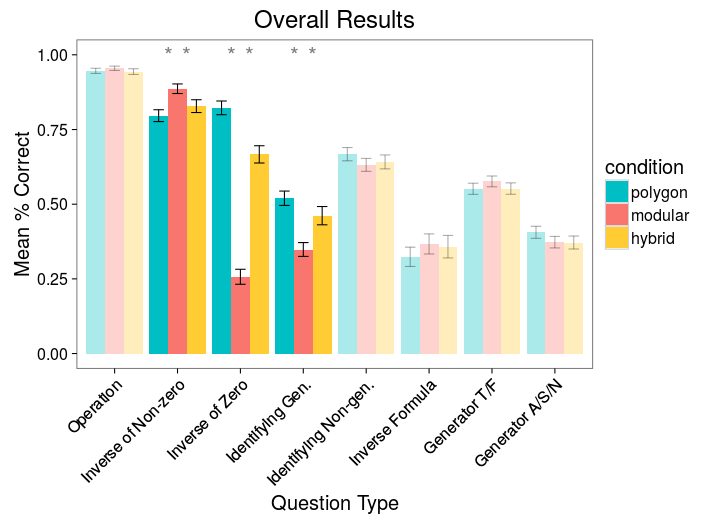
\includegraphics[width=0.8\textwidth]{figures/overall_results.png}
\caption{Results aggregated across group orders and all three experiments}
\label{overall_results}
\end{figure*}
Overall, performance was quite high on the basic operation questions and declined on the questions about inverses and generators. Performance was similar across the order 6 and order 9 groups, but declined substantially in the order $n$ group, suggesting that the subjects were able to transfer their procedures for solving the questions to a different group order, but were not able to formally express them in a generic way. \par
The polygon group and the modular group differed significantly on a number of question types, with the polygon group consistently performing better at identifying elements that were generators and finding the inverse of zero, while the modular group performed significantly better at finding the inverse of non-zero elements. See fig. \ref{overall_results} for a summary of the results aggregated across experiments and group orders (but note that this understates the hybrid group's performance, because the hybrid group showed an improvement on a number of aspects of understanding between the order 6 and order 9 questions). For a full presentation of the results, see below and the supplemental figures appendix.  
\FloatBarrier
\subsection{Full Results}
\subsubsection{Operation}
\begin{figure*}[t]
\centering
\begin{subfigure}[c]{0.4\textwidth}
\centering
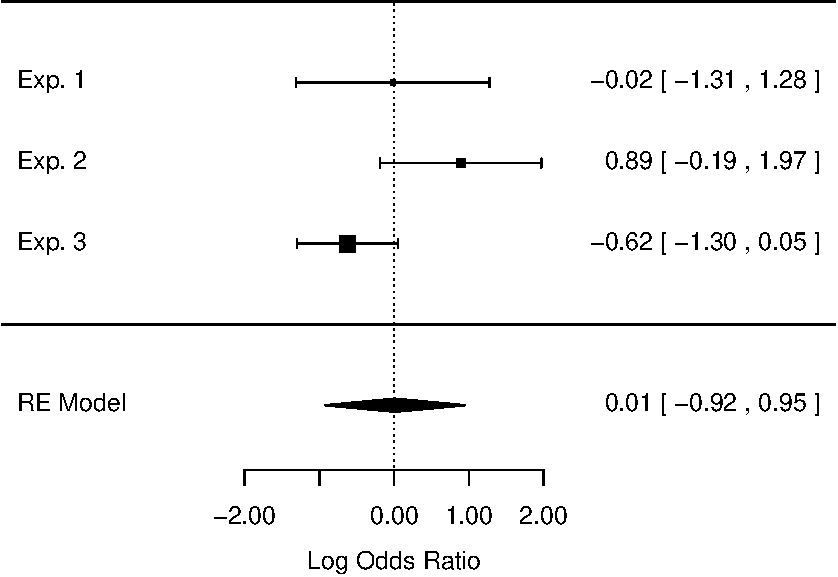
\includegraphics[width=\textwidth]{figures/meta/conditionpolygon.pdf}
\caption{Order 6}
\end{subfigure}
~
\begin{subfigure}[c]{0.4\textwidth}
\centering
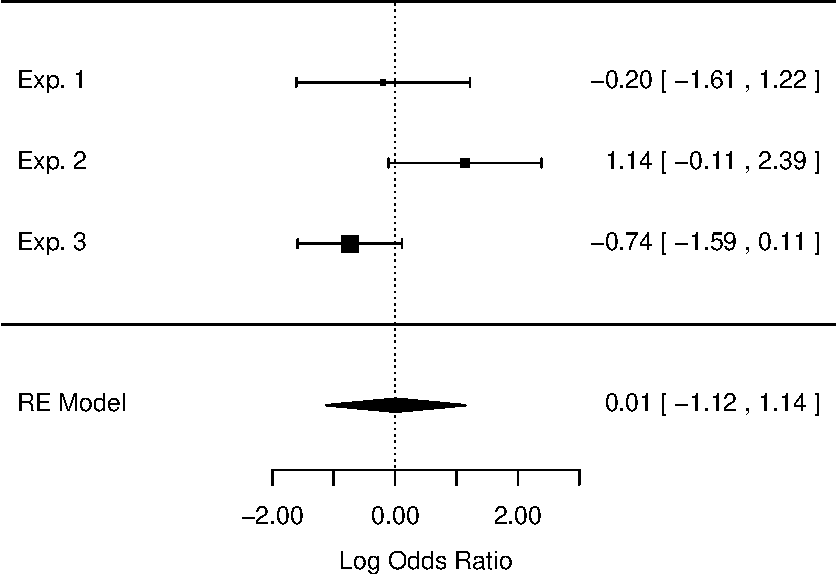
\includegraphics[width=\textwidth]{figures/meta/question_typeoperation_9_conditionpolygon.pdf}
\caption{Order 9}
\end{subfigure}
\caption{Meta analysis -- polygon vs. modular, operation}
\label{meta_op_p}
\end{figure*}\noindent 

\begin{figure*}[t]
\centering
\begin{subfigure}[c]{0.4\textwidth}
\centering
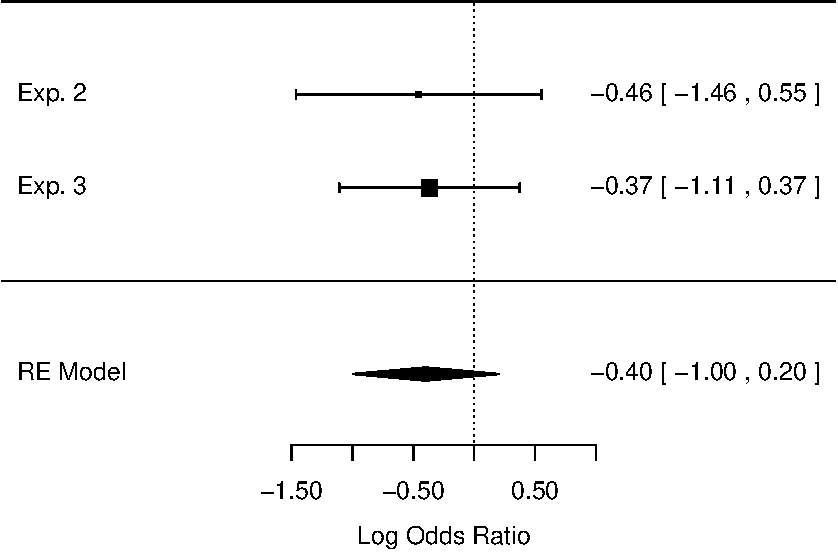
\includegraphics[width=\textwidth]{figures/meta/conditionhybrid.pdf}
\caption{Order 6}
\end{subfigure}
~
\begin{subfigure}[c]{0.4\textwidth}
\centering
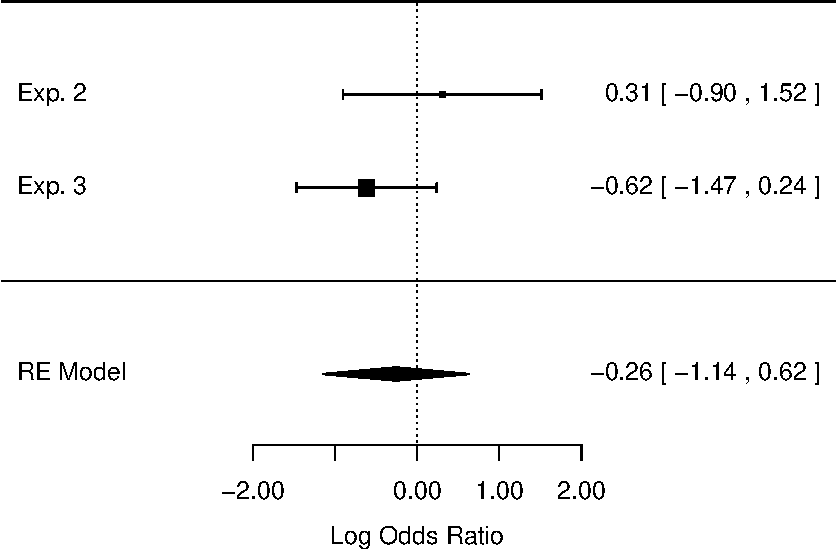
\includegraphics[width=\textwidth]{figures/meta/question_typeoperation_9_conditionhybrid.pdf}
\caption{Order 9}
\end{subfigure}
\caption{Meta analysis -- hybrid vs. modular, operation}
\label{meta_op_h}
\end{figure*}\noindent 
\textit{Experiment 1:} There was no significant difference in the performance on the basic operation questions between the experimental groups (see Figure \ref{ex1_op}) in either the order 6 group ($\beta = 0.006$, $t = 0.18$, $p = 0.86$) or the order 9 group ($\beta = -0.009$, $t = -0.26$, $p = 0.79$). These are the questions where the wording varied in accordance with the different representations taught to the experimental groups. Both groups performed quite well, with over 90\% accuracy. \par 
\textit{Experiment 2:} We replicated our result that there was no significant difference in the performance on the basic operation questions between the modular and polygon experimental groups (see Figure \ref{ex2_op}) in either group order (order 6: $\beta = 0.02$, $t = 0.735$, $p = 0.46$; order 9: $\beta = 0.02$, $t = 0.63$, $p = 0.53$). Furthermore, there was no significant difference between the hybrid and modular groups (order 6: $\beta = -0.02$, $t = -0.72$, $p = 0.47$; order 9: $\beta = 0.04$, $t = 1.10$, $p = 0.27$).\par
\textit{Experiment 3:} We replicated our result that there was no significant difference in the performance on the basic operation questions between the modular and polygon experimental groups (see Figure \ref{ex3_op}) in either group order (order 6: $\beta$ 95\%-CI = $[-2.55,0.15]$, $p > 0.05$; order 9: $\beta$ 95\%-CI = $[-1.59,0.11]$, $p > 0.05$), and our result that there was no significant difference between the hybrid and modular groups (order 6:  $\beta$ 95\%-CI = $[-2.13,0.13]$, $p > 0.05$; order 9: $\beta$ 95\%-CI = $[-1.90,0.17]$, $p > 0.05$). \par
\textit{Meta-Analysis:} We estimate any effect of the polygon presentation on the ability to perform the group operation to be small (order 6: log OR = 0.01; order 9: log OR = 0.01; see fig. \ref{meta_op_p}). We estimate any effect of the hybrid presentation on the ability to perform the group operation to be small (order 6: log OR = -0.40; order 9: log OR = -0.26; see fig. \ref{meta_op_h}).\par
\textit{Summary:} Despite learning different methods for performing the group operation, the experimental groups do not differ substantially in their ability to perform it. 
\FloatBarrier
\subsubsection{Inverses}
\begin{figure*}
\centering
\begin{subfigure}[c]{0.4\textwidth}
\centering
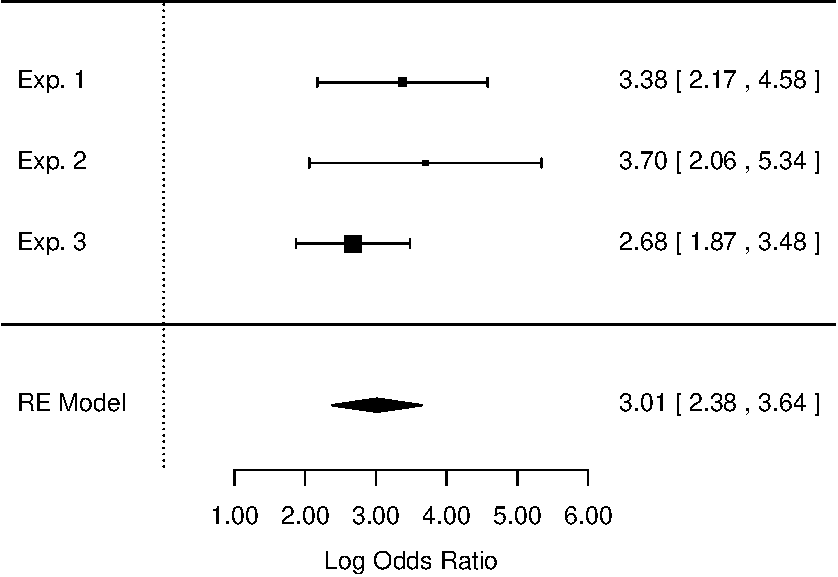
\includegraphics[width=\textwidth]{figures/meta/question_typeinverse_zero_6_conditionpolygon.pdf}
\caption{Order 6}
\end{subfigure}
~
\begin{subfigure}[c]{0.4\textwidth}
\centering
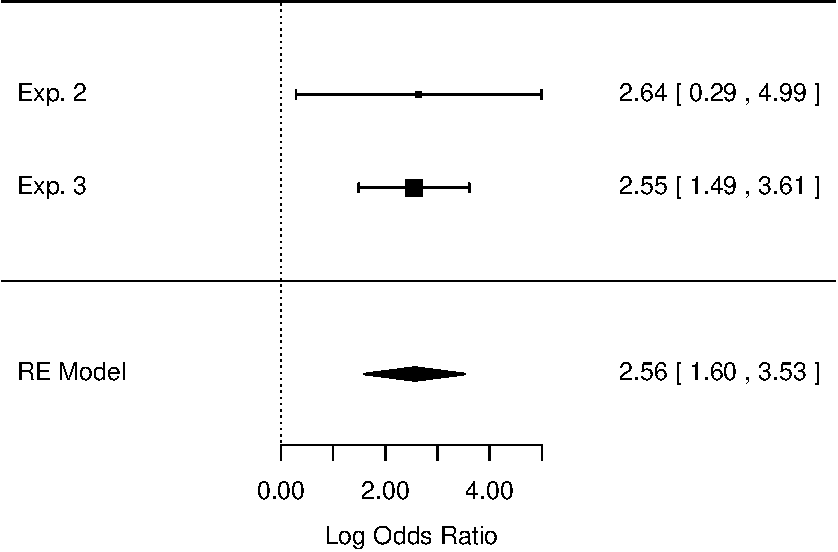
\includegraphics[width=\textwidth]{figures/meta/question_typeinverse_zero_9_conditionpolygon.pdf}
\caption{Order 9}
\end{subfigure}
\caption{Meta analysis -- polygon vs. modular, inverse of zero}
\label{meta_inZ_p}
\end{figure*}\noindent 

\begin{figure*}
\centering
\begin{subfigure}[c]{0.4\textwidth}
\centering
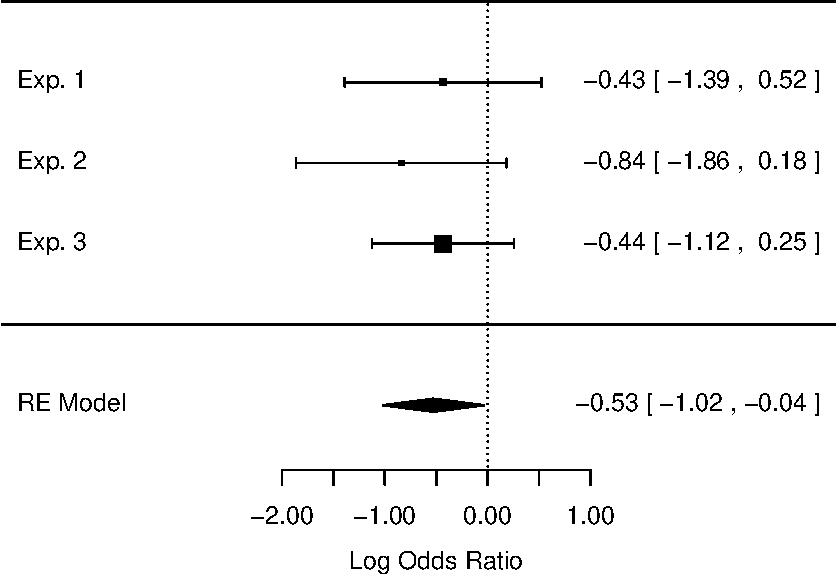
\includegraphics[width=\textwidth]{figures/meta/question_typeinverse_nonzero_6_conditionpolygon.pdf}
\caption{Order 6}
\end{subfigure}
~
\begin{subfigure}[c]{0.4\textwidth}
\centering
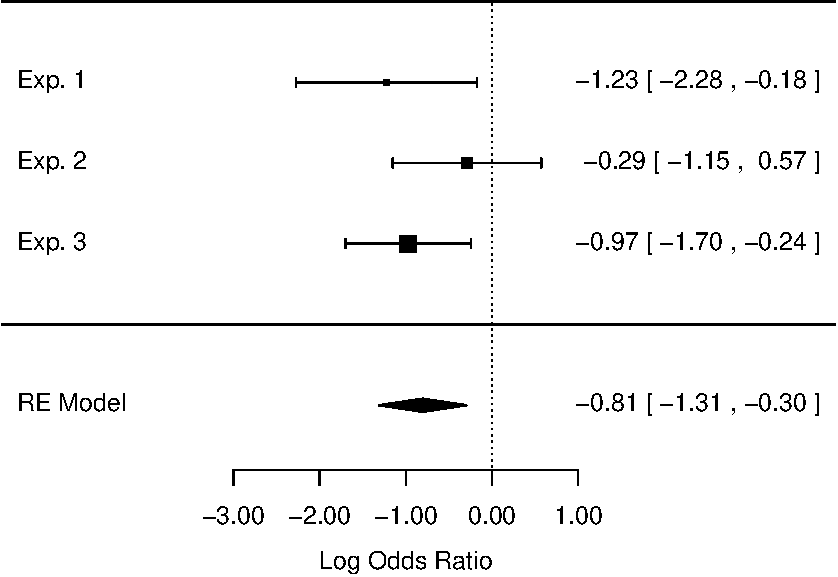
\includegraphics[width=\textwidth]{figures/meta/question_typeinverse_nonzero_9_conditionpolygon.pdf}
\caption{Order 9}
\end{subfigure}
\caption{Meta analysis -- polygon vs. modular, inverse of non-zero}
\label{meta_inNZ_p}
\end{figure*}\noindent 
\begin{figure*}
\centering
\begin{subfigure}[c]{0.4\textwidth}
\centering
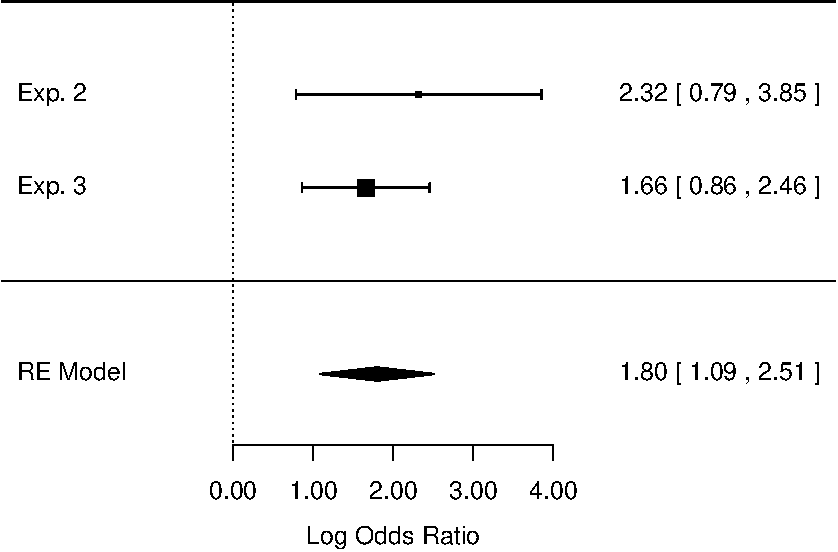
\includegraphics[width=\textwidth]{figures/meta/question_typeinverse_zero_6_conditionhybrid.pdf}
\caption{Order 6}
\end{subfigure}
~
\begin{subfigure}[c]{0.4\textwidth}
\centering
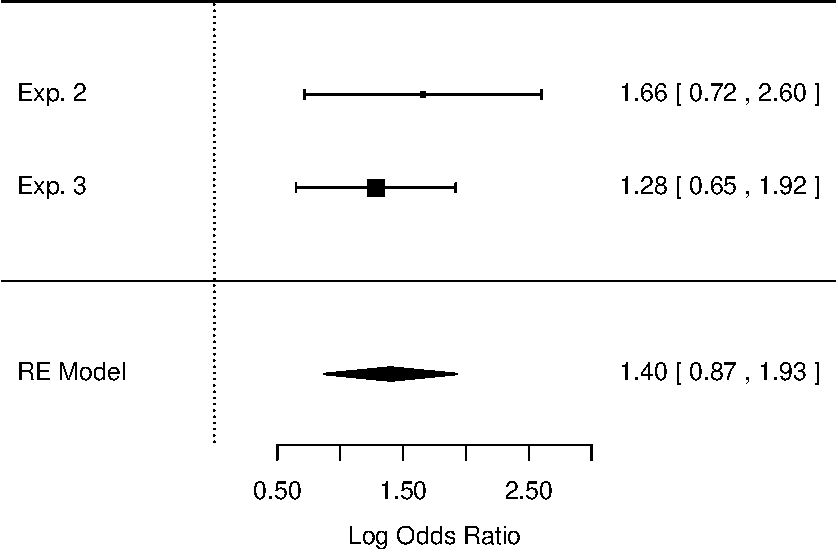
\includegraphics[width=\textwidth]{figures/meta/question_typeinverse_zero_9_conditionhybrid.pdf}
\caption{Order 9}
\end{subfigure}
\caption{Meta analysis -- hybrid vs. modular, inverse of zero}
\label{meta_inZ_h}
\end{figure*}\noindent 

\begin{figure*}
\centering
\begin{subfigure}[c]{0.4\textwidth}
\centering
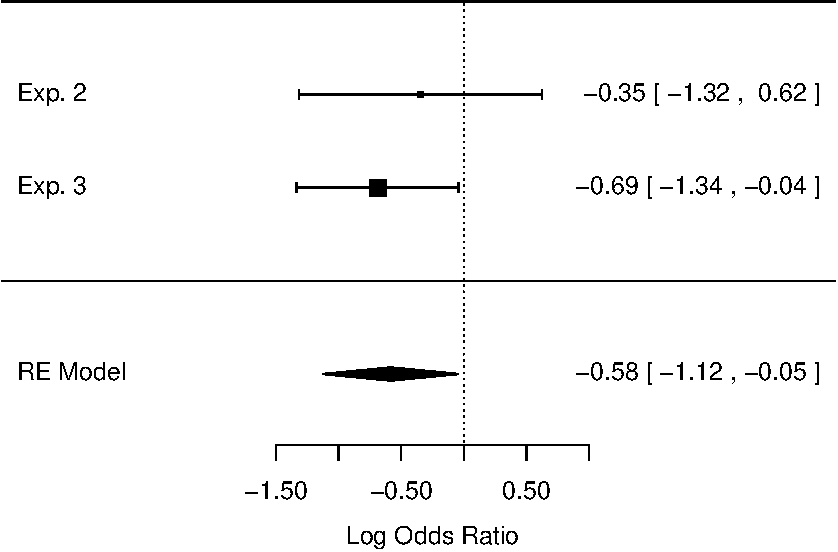
\includegraphics[width=\textwidth]{figures/meta/question_typeinverse_nonzero_6_conditionhybrid.pdf}
\caption{Order 6}
\end{subfigure}
~
\begin{subfigure}[c]{0.4\textwidth}
\centering
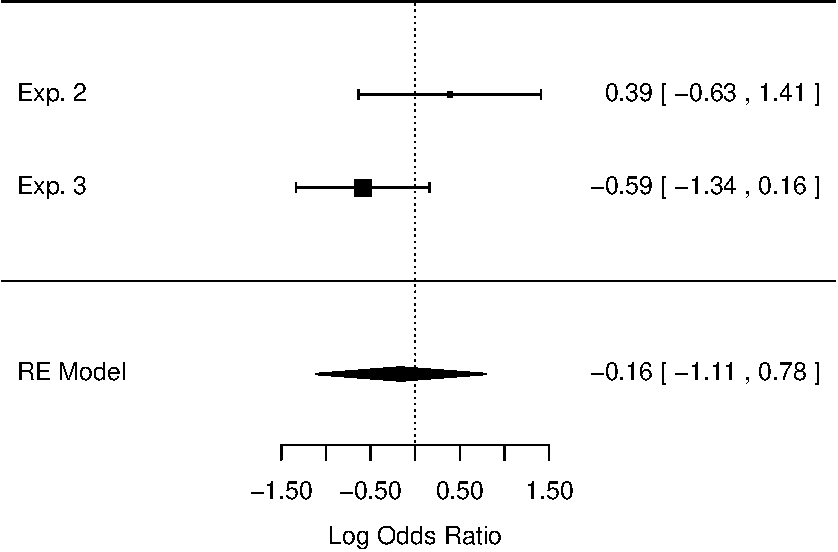
\includegraphics[width=\textwidth]{figures/meta/question_typeinverse_nonzero_9_conditionhybrid.pdf}
\caption{Order 9}
\end{subfigure}
\caption{Meta analysis -- hybrid vs. modular, inverse of non-zero}
\label{meta_inNZ_h}
\end{figure*}\noindent 

\begin{figure*}
\centering
\begin{subfigure}[c]{0.4\textwidth}
\centering
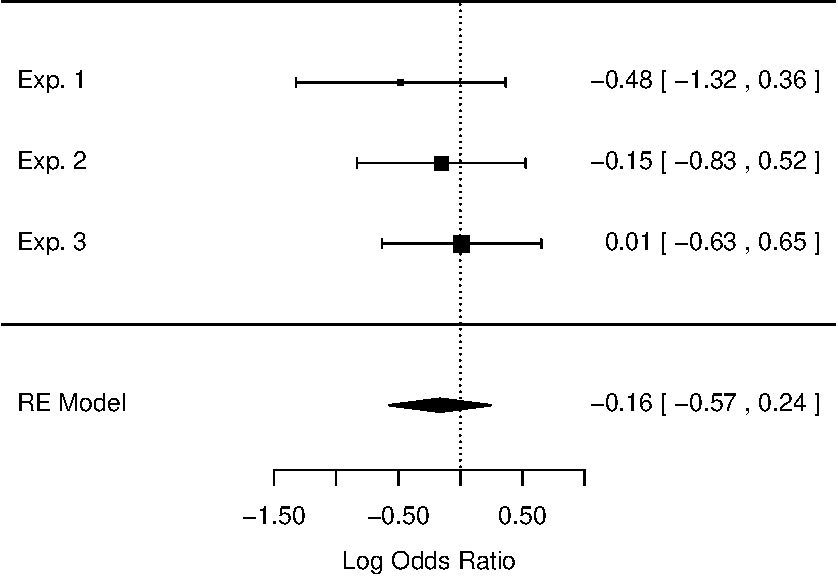
\includegraphics[width=\textwidth]{figures/meta/question_typeinverse_formula_n_conditionpolygon.pdf}
\caption{Polygon vs. modular}
\end{subfigure}
~
\begin{subfigure}[c]{0.4\textwidth}
\centering
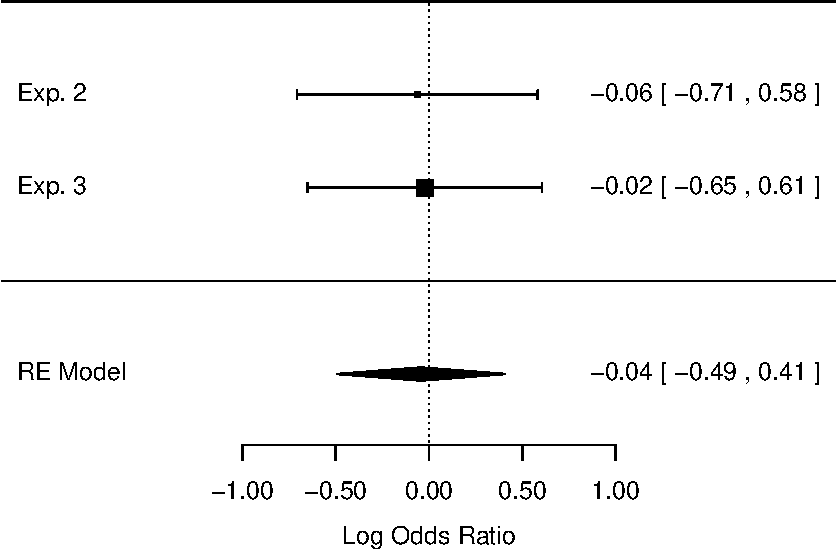
\includegraphics[width=\textwidth]{figures/meta/question_typeinverse_formula_n_conditionhybrid.pdf}
\caption{Hybrid vs. modular}
\end{subfigure}
\caption{Meta analysis -- inverse formula}
\label{meta_in_f}
\end{figure*}\noindent 
\textit{Experiment 1:} For inverses the polygon group was significantly worse at finding the inverse of non-zero elements in the order 9 group ($\beta = -0.169$, $t=-3.73$, $p < 0.001$), but better at finding the inverse of zero (see Figure \ref{ex1_in}) in the order 6 group ($\beta = 0.66$, $t=9.13$, $p < 0.001$). (Unfortunately we did not include an inverse of zero question in the order 9 group in this experiment, so we only have data from the order 6 group.) The modular group was significantly better at writing the generic formulas for the inverse of 1 and an arbitrary element $x$ in the group of order $n$ ($\beta = -0.11$, $t=-1.99$, $p = 0.047$). \par
\textit{Experiment 2:}  We replicated our results that the modular group performed better at inverses of non-zero elements (order 6: $\beta = -0.11$, $t = -2.59$, $p = 0.009$; order 9: $\beta = -0.07$, $t = -1.48$, $p = 0.13$), and the polygon group performed better at inverse of zero questions (order 6: $\beta = 0.68$, $t = 8.842$, $p < 0.001$; order 9: $\beta = 0.44$, $t = 5.80$, $p < 0.001$). (Note that the modular group performed worse than the polygon group even in the order 9 group, once they had already seen an example of an inverse of zero with feedback.) The polygon group did not perform significantly differently from the modular group at the inverse formula questions ($\beta = -0.05$, $t=-0.94$, $p = 0.35$). The hybrid group did not perform significantly worse than the modular group at inverses of non-zero elements (order 6: $\beta = -0.007$, $t = -0.173$, $p = 0.86$; order 9: $\beta = 0.08$, $t = 1.56$, $p = 0.12$), and did perform significantly better at inverses of zero (order 6: $\beta = 0.46$, $t = 5.95$, $p < 0.001$; order 9: $\beta = 0.38$, $t = 4.91$, $p < 0.001$). However, it is clear that the hybrid group is not initially performing as well as the polygon group on this question, so there is still room for improvement. The hybrid group did not perform significantly differently from the modular group at the inverse formula questions ($\beta = 0.01$, $t=0.125$, $p =0.90$). (See Figure \ref{ex2_in}.) \par 
\textit{Experiment 3:} We replicated our results that the modular group performed better than the polygon group at inverses of non-zero elements only in the order 9 group, although the effect was in the correct direction in the order 6 group (order 6: $\beta$ 95\%-CI = $[-1.14,0.24]$, $p > 0.05$; order 9: $\beta$ 95\%-CI = $[-1.74,-0.27]$, $p < 0.05$). We replicated our result that the polygon group performed better at inverse of zero questions (order 6: $\beta$ 95\%-CI = $[1.93,3.55]$, $p < 0.05$; order 9: $\beta$ 95\%-CI = $[1.72,3.60]$, $p < 0.05$). The polygon group did not perform significantly differently from the modular group at the inverse formula questions ($\beta$ 95\%-CI = $[-0.64,0.65]$, $p > 0.05$). The hybrid group was not significantly worse than the modular group at inverses of non-zero elements in either group, although it was trending worse in the order 6 group (order 6: $\beta$ 95\%-CI = $[-1.92,0.01]$, $p > 0.05$; order 9: $\beta$ 95\%-CI = $[-1.96,0.24]$, $p > 0.05$). We replicated our result that the hybrid group was significantly better at inverses of zero only in the order 6 group, although the effect was trending in the order 9 group (order 6: $\beta$ 95\%-CI = $[0.21,2.65]$, $p < 0.05$; order 9: $\beta$ 95\%-CI = $[-0.01,2.09]$, $p > 0.05$).The polygon group did not perform significantly differently from the modular group at the inverse formula questions ($\beta$ 95\%-CI = $[-1.32,0.78]$, $p > 0.05$) (See Figure \ref{ex3_in}.) \par
\textit{Meta-Analysis:} We estimated the positive effect of the polygon condition on inverse of zero questions to be large for both group orders, although the effect is smaller for order 9, consistent with some learning in the modular group (order 6: log OR = 3.01; order 9: log OR = 2.56; see fig. \ref{meta_inZ_p}). We estimated the negative effect of the polygon condition on inverse of non-zero questions to be moderately sized (order 6: log OR = -0.53; order 9: log OR = -0.81; see fig. \ref{meta_inNZ_p}). We estimated the positive effect of the hybrid condition on inverse of zero questions to be large for both group orders, although it is not as large as that of the polygon condition, and the effect is smaller for order 9, consistent with some learning in the modular group (order 6: log OR = 1.80; order 9: log OR = 1.40; see fig. \ref{meta_inZ_h}). We estimated the negative effect of the hybrid condition on inverse of non-zero questions to be moderately sized and possibly vanishing after further practice in the order 9 group (order 6: log OR = -0.58; order 9: log OR = -0.16; see fig. \ref{meta_inNZ_h}). We estimated the effect of the polygon condition on the inverse formula questions to be neglible (log OR = -0.16, see fig. \ref{meta_in_f}), and similarly for the effect of the hybrid condition on the inverse formula questions (log OR = -0.04, see fig. \ref{meta_in_f}). \par
\textit{Summary:} Overall, it seems that the modular presentation is generally beneficial for finding inverses, except in the case of zero, where the polygon presentation subjects perform much better. (See discussion for a possible explanation of this result.) 
\FloatBarrier
\subsubsection{Generators}
\begin{figure*}
\centering
\begin{subfigure}[c]{0.4\textwidth}
\centering
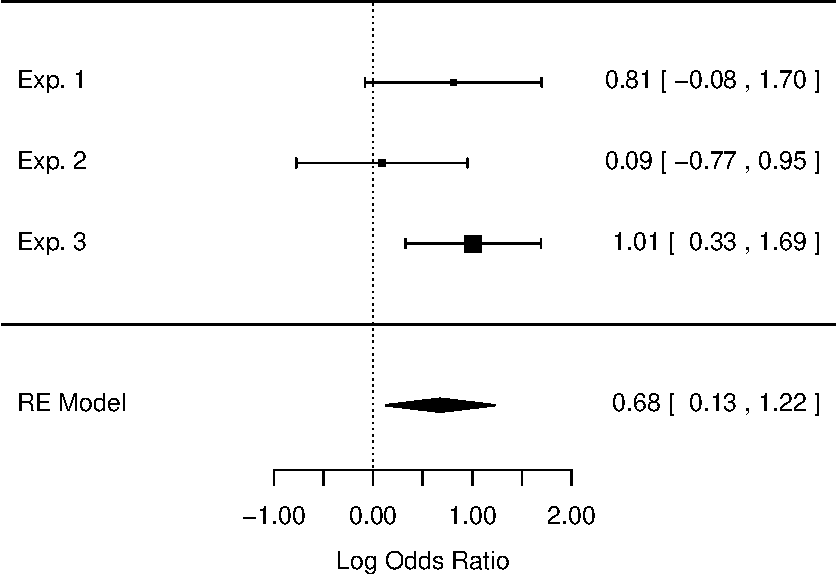
\includegraphics[width=\textwidth]{figures/meta/question_typegenerator_true_6_conditionpolygon.pdf}
\caption{Order 6}
\end{subfigure}
~
\begin{subfigure}[c]{0.4\textwidth}
\centering
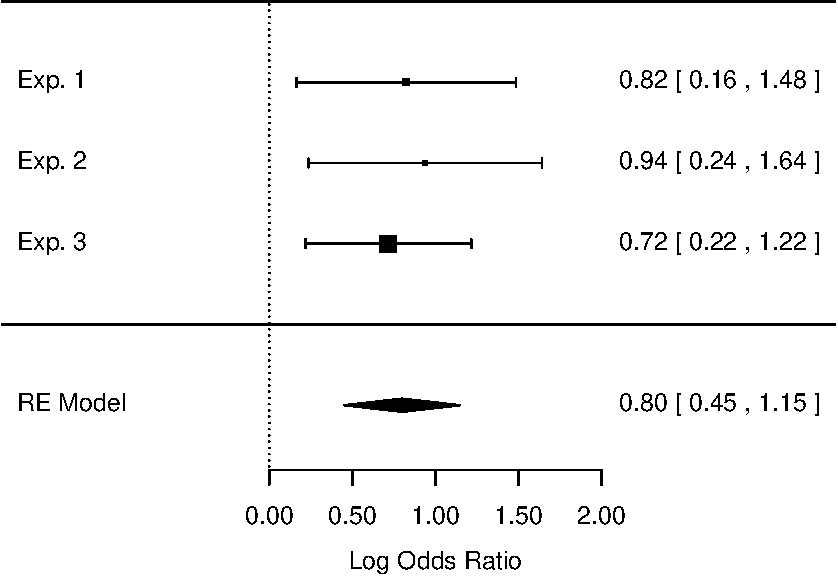
\includegraphics[width=\textwidth]{figures/meta/question_typegenerator_true_9_conditionpolygon.pdf}
\caption{Order 9}
\end{subfigure}
\caption{Meta analysis -- polygon vs. modular, identifying generators}
\label{meta_genT_p}
\end{figure*}\noindent 

\begin{figure*}
\centering
\begin{subfigure}[c]{0.4\textwidth}
\centering
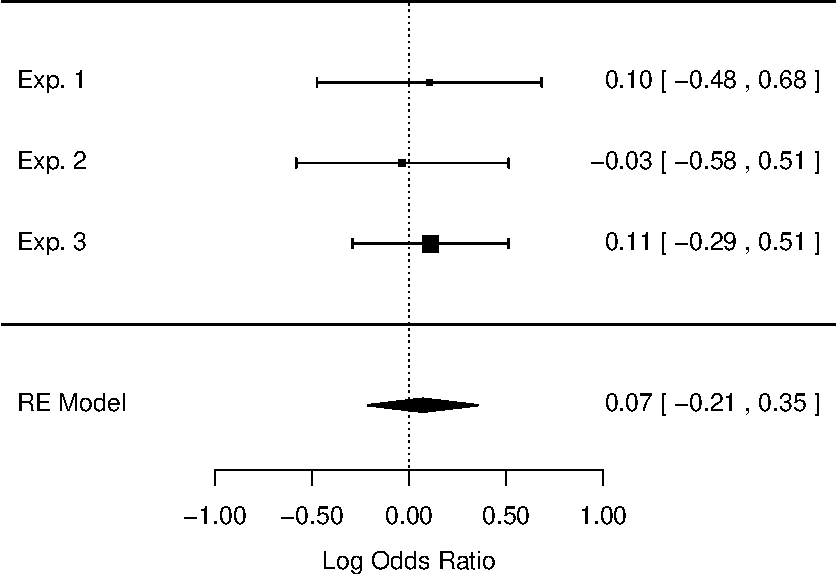
\includegraphics[width=\textwidth]{figures/meta/question_typegenerator_false_6_conditionpolygon.pdf}
\caption{Order 6}
\end{subfigure}
~
\begin{subfigure}[c]{0.4\textwidth}
\centering
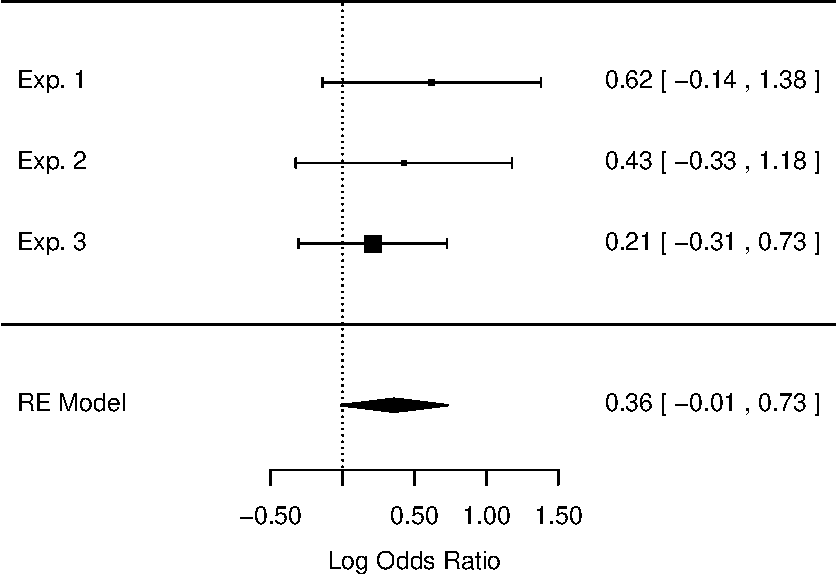
\includegraphics[width=\textwidth]{figures/meta/question_typegenerator_false_9_conditionpolygon.pdf}
\caption{Order 9}
\end{subfigure}
\caption{Meta analysis -- polygon vs. modular, identifying non-generators}
\label{meta_genF_p}
\end{figure*}\noindent 

\begin{figure*}
\centering
\begin{subfigure}[c]{0.4\textwidth}
\centering
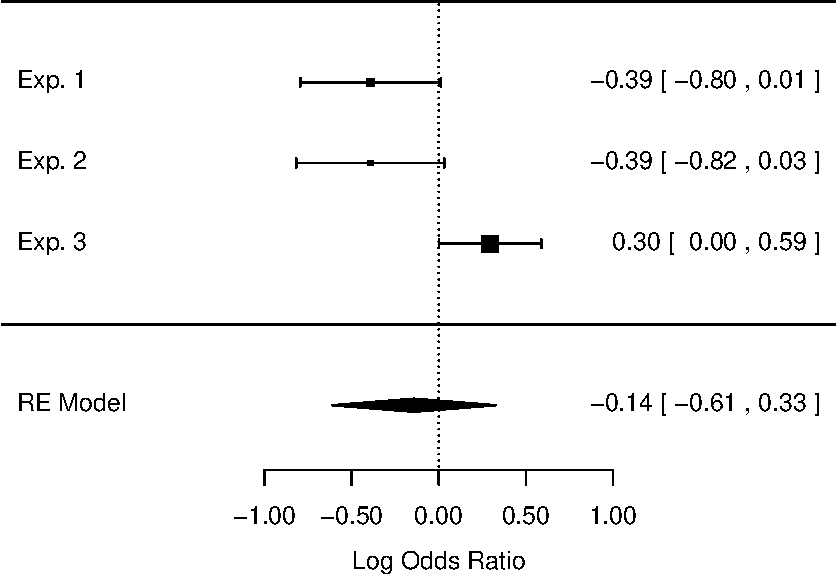
\includegraphics[width=\textwidth]{figures/meta/question_typegenerator_TF_n_conditionpolygon.pdf}
\caption{T/F}
\end{subfigure}
~
\begin{subfigure}[c]{0.4\textwidth}
\centering
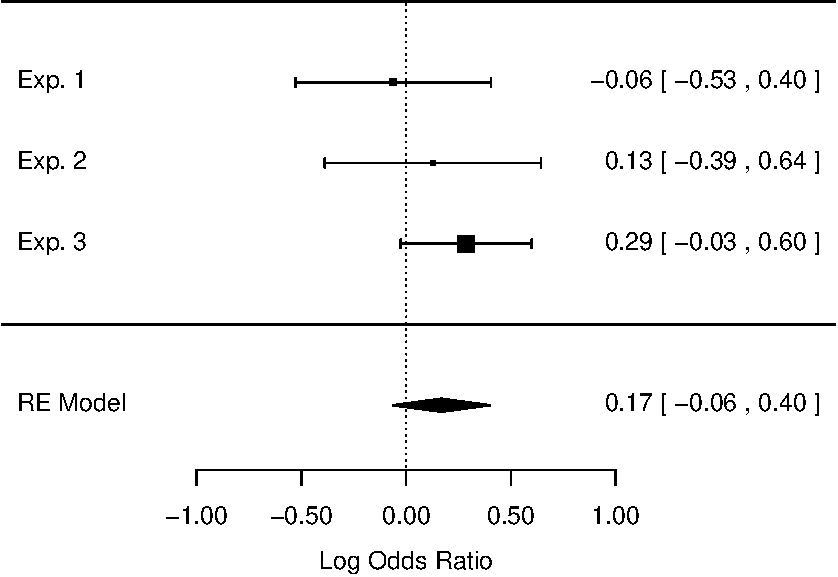
\includegraphics[width=\textwidth]{figures/meta/question_typegenerator_ASN_n_conditionpolygon.pdf}
\caption{A/S/N}
\end{subfigure}
\caption{Meta analysis -- polygon vs. modular, generator t/f \& a/s/n}
\label{meta_genTF_p}
\end{figure*}\noindent 
\begin{figure*}
\centering
\begin{subfigure}[c]{0.4\textwidth}
\centering
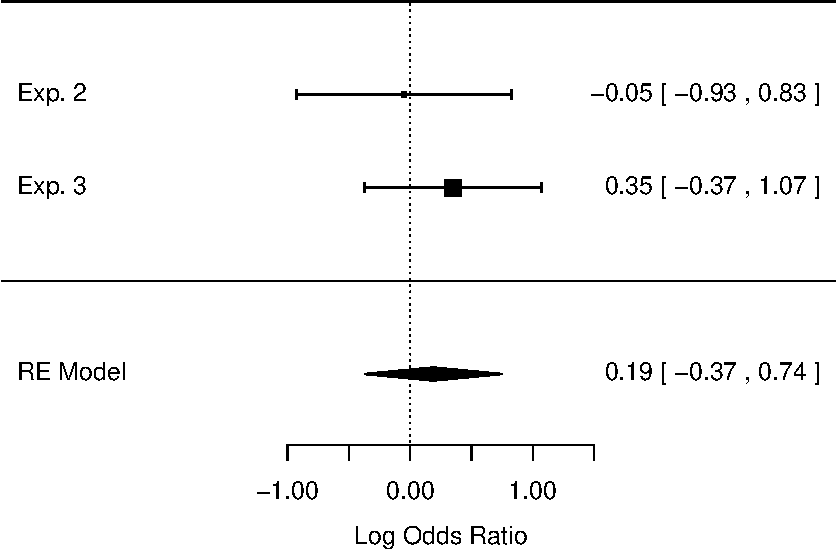
\includegraphics[width=\textwidth]{figures/meta/question_typegenerator_true_6_conditionhybrid.pdf}
\caption{Order 6}
\end{subfigure}
~
\begin{subfigure}[c]{0.4\textwidth}
\centering
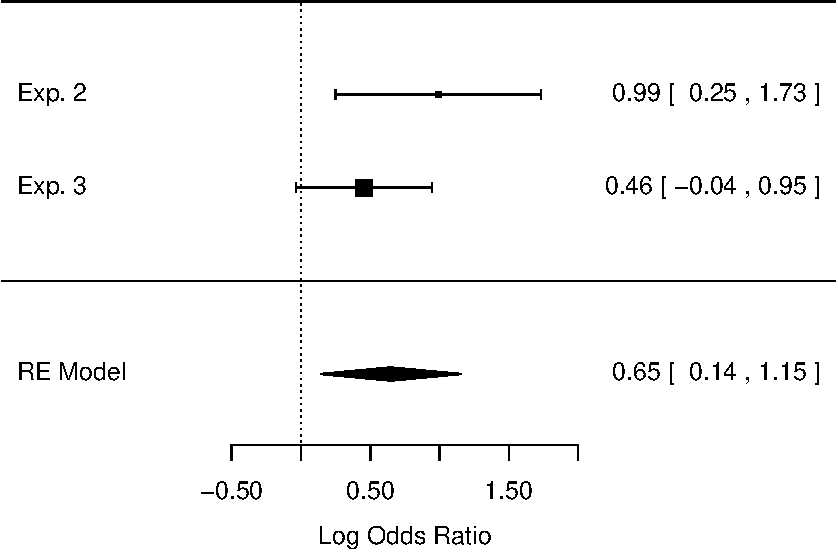
\includegraphics[width=\textwidth]{figures/meta/question_typegenerator_true_9_conditionhybrid.pdf}
\caption{Order 9}
\end{subfigure}
\caption{Meta analysis -- hybrid vs. modular, identifying generators}
\label{meta_genT_h}
\end{figure*}\noindent 

\begin{figure*}
\centering
\begin{subfigure}[c]{0.4\textwidth}
\centering
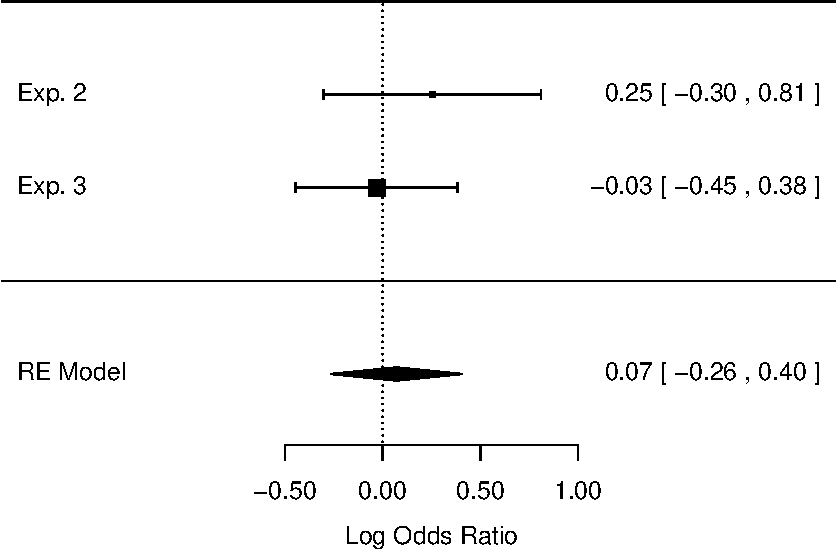
\includegraphics[width=\textwidth]{figures/meta/question_typegenerator_false_6_conditionhybrid.pdf}
\caption{Order 6}
\end{subfigure}
~
\begin{subfigure}[c]{0.4\textwidth}
\centering
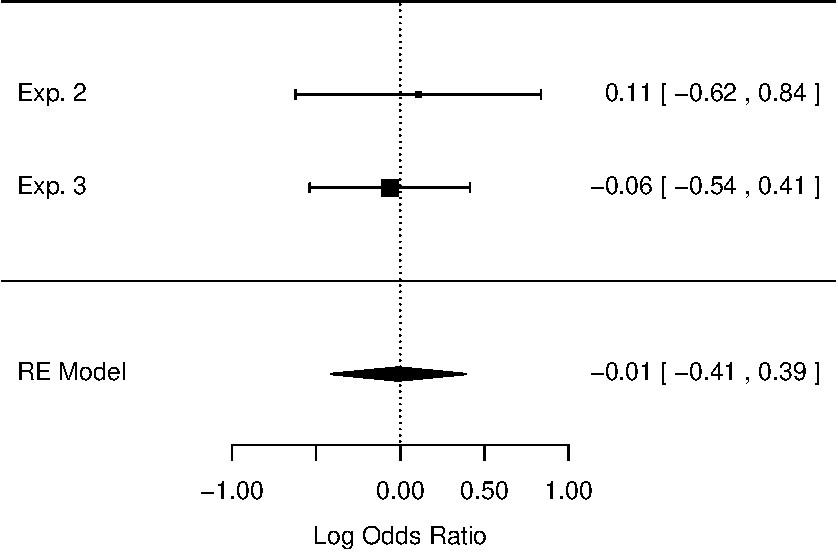
\includegraphics[width=\textwidth]{figures/meta/question_typegenerator_false_9_conditionhybrid.pdf}
\caption{Order 9}
\end{subfigure}
\caption{Meta analysis -- hybrid vs. modular, identifying non-generators}
\label{meta_genF_h}
\end{figure*}\noindent 

\begin{figure*}
\centering
\begin{subfigure}[c]{0.4\textwidth}
\centering
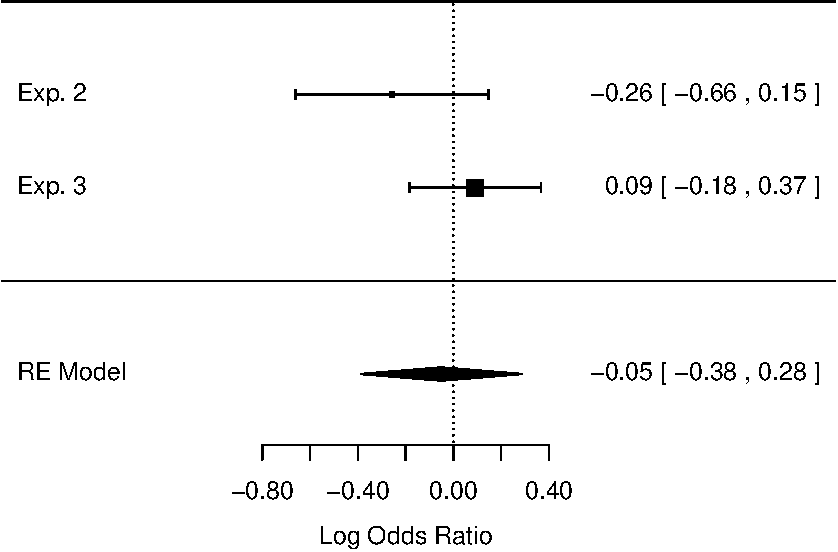
\includegraphics[width=\textwidth]{figures/meta/question_typegenerator_TF_n_conditionhybrid.pdf}
\caption{T/F}
\end{subfigure}
~
\begin{subfigure}[c]{0.4\textwidth}
\centering
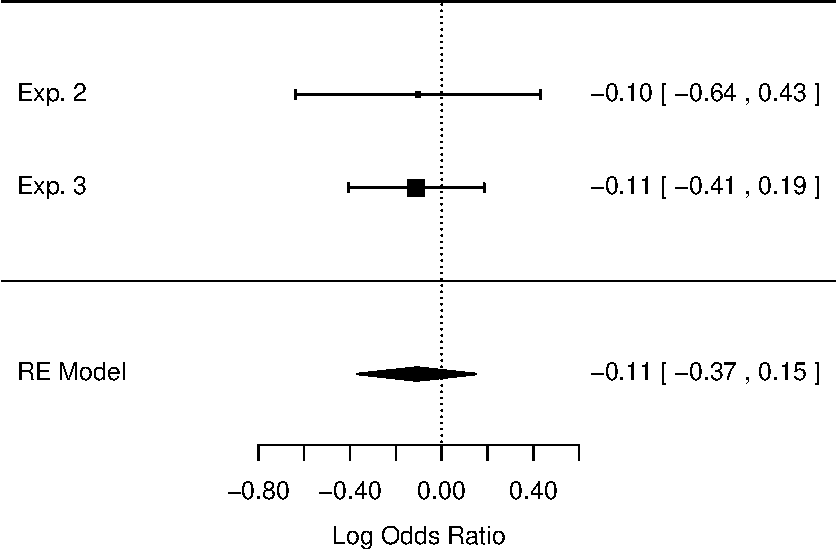
\includegraphics[width=\textwidth]{figures/meta/question_typegenerator_ASN_n_conditionhybrid.pdf}
\caption{A/S/N}
\end{subfigure}
\caption{Meta analysis -- hybrid vs. modular, generator T/F \& A/S/N}
\label{meta_genTF_h}
\end{figure*}\noindent 
\textit{Experiment 1:} The polygon group performed significantly better at identifying elements that were generators (order 6: $\beta = 0.164$, $t = 2.27$, $p = 0.02$; order 9: $\beta = 0.184$, $t = 3.45$, $p < 0.001$). The groups did not differ significantly at identifying non-generators in the order 6 group, but the polygon group performed significantly better in the order 9 group (order 6: $\beta = 0.01$, $t = 0.235$, $p = 0.81$; order 9: $\beta = 0.12$, $t = 2.32$, $p = 0.02$). The modular group performed better at the T/F questions about generators in the order $n$ group ($\beta = -0.11$, $t = -2.60$, $p = 0.009$). However, performance on these questions was not too far above chance. The groups did not differ significantly on the A/S/N questions ($\beta = -0.03$, $t = -0.5$, $p = 0.62$). (See Figure \ref{ex1_gen}.)\par
\textit{Experiment 2:} We replicated our result that the polygon group is better at identifying generators only in the order 9 group (order 6: $\beta = 0.00$, $t = -0.05$, $p = 1.00$; order 9: $\beta = 0.19$, $t = 3.37$, $p < 0.001$), and the polygon group did not perform better at identifying non-generators in either group (order 6: $\beta = -0.03$, $t = -0.60$, $p = 0.55$; order 9: $\beta = 0.07$, $t = 1.31$, $p = 0.19$). We replicated our result that the modular group performed better at T/F questions about generators ($\beta = -0.12$, $t = -2.71$, $p = 0.007$). We replicated our result that the polygon and modular groups did not significantly differ at the A/S/N questions ($\beta =  0.01$, $t = 0.139$, $p = 0.89$). The hybrid group perfomed significantly better than the modular group at identifying generators in the group order where our previous finding replicated ($\beta = 0.25$, $t = 4.31$, $p < 0.001$), did not significantly differ at identify non-generators (order 6: $\beta = 0.07$, $t = 1.51$, $p = 0.13$; order 9: $\beta = 0.05$, $t = 0.80$, $p = 0.42$), and did not perform significantly worse at the T/F questions ($\beta = -0.042$, $t = -0.98$, $p = 0.33$). However, it appears that the hybrid group did not be achieve performance completely on par with the modular group on the T/F questions. The hybrid and modular groups did not differ significantly on the A/S/N questions ($\beta = -0.00$, $t = -0.01$, $p = 0.99$). (See Figure \ref{ex2_gen}.) \par
\textit{Experiment 3:} We replicated our result that the polygon group is better at identifying generators (order 6: $\beta$ 95\%-CI = $[0.35,1.72]$, $p < 0.05$; order 9: $\beta$ 95\%-CI = $[0.22,1.22]$, $p < 0.05$), and that the polygon group did not significantly differ from the modular at identifying non-generators (order 6: $\beta$ 95\%-CI = $[-0.29,0.50]$, $p > 0.05$; order 9: $\beta$ 95\%-CI = $[-0.32,0.73]$, $p > 0.05$). We failed to replicate our result that the modular group is better than the polygon group at T/F questions about generators, in fact the polygon group performed significantly better in this experiment ($\beta$ 95\%-CI = $[0.004,0.59]$, $p < 0.05$). We replicated our result that the polygon and modular groups did not differ significantly at answering A/S/N questions ($\beta$ 95\%-CI = $[-0.03,0.60]$, $p > 0.05$). We failed to replicate our result that the hybrid group is significantly better than the modular group at identifying generators in either group order, although both effects were slightly in that direction (order 6: $\beta$ 95\%-CI = $[-1.11,1.27]$, $p > 0.05$; order 9: $\beta$ 95\%-CI = $[-0.78, 1.17]$, $p > 0.05$). We replicated our result that the hybrid group did not significantly differ at identifying non-generators (order 6: $\beta$ 95\%-CI = $[-1.17,0.60]$, $p > 0.05$; order 9: $\beta$ 95\%-CI = $[-1.25,0.61]$, $p > 0.05$). We replicated our result that the modular and hybrid groups did not significantly differ at the T/F questions ($\beta$ 95\%-CI = $[-1.05, 0.71]$, $p > 0.05$). We replicated our result that the modular and hybrid groups did not significantly differ at the A/S/N questions ($\beta$ 95\%-CI = $[-1.26,0.53]$, $p > 0.05$). (See Figure \ref{ex3_gen}.) \par
\textit{Meta-Analysis:}  We estimated the positive effect of the polygon condition on identifying generators to be moderately sized (order 6: log OR = 0.68; order 9: log OR = 0.80; see fig. \ref{meta_genT_p}). We estimated the effect of the polygon condition on identifying non-generators to be small, but maybe slightly positive in the group of order 9 (order 6: log OR = 0.07; order 9: log OR = 0.36; see fig. \ref{meta_genF_p}). We estimated that any effect of the polygon condition on answering True/False questions about generators is small (log OR = -0.14; see fig. \ref{meta_genTF_p}). We estimated that any effect of the polygon condition on answering Always/Sometimes/Never questions about generators is small (log OR = 0.17; see fig. \ref{meta_genTF_p}). We estimated the positive effect of the hybrid condition on identifying generators to be small in the order 6 group, but increasing in the order 9 group, (order 6: log OR = 0.19; order 9: log OR = 0.65; see fig. \ref{meta_genT_h}). We estimated the effect of the hybrid condition on identifying non-generators to be small (order 6: log OR = 0.07; order 9: log OR = -0.01; see fig. \ref{meta_genF_h}). We estimated the effect of the hybrid condition on answering True/False questions about generators to be small (log OR = -0.05; see fig. \ref{meta_genTF_h}). We estimated the effect of the hybrid condition on answering Always/Sometimes/Never questions about generators to be small (log OR = -0.11; see fig. \ref{meta_genTF_h}).\par
\textit{Summary:} Overall, it seems that the polygon presentation is beneficial for identifying generators, and the hybrid presentation seems to be similarly beneficial for identifying generators in the order 9 group, once they have had some practice. None of the presentations seem particularly beneficial for identifying non-generators, or for answering T/F or A/S/N questions about generators, performance was quite low on these questions.
\FloatBarrier
\subsection{Other Analyses}
We conducted several other analyses to further elucidate the differences in performance between the groups, and the cognitive factors underlying them.\\
\subsubsection{Diagram use}
We hypothesized that the polygon group's superior performance on identifying generators might be due to the ability to use the spatial structure of the polygon to more easily visualize the elements generated by an element (see discussion). One possible prediction of this hypothesis would be that within the polygon group, interaction with the diagram might be predictive of success on these questions. (Of course, we could only record the interactions with the mouse, while many subjects may have just gazed or pointed at the diagram to use it in their thinking. Furthermore, the use of the diagram may be confounded with overall engagement. Our results must be interpreted with this in mind.) \par
We performed a mixed-model logistic regression on data from the polygon and hybrid subjects from Experiments 2 and 3, predicting correct answers by whether or not they used the diagram (and a random effect of subject). We found that using the diagram was significantly predictive of success on the questions (Exp. 2: $\beta=1.90$, $z = 2.76$, $p = 0.006$; Exp. 3: $\beta=2.24$, $z = 5.12$, $p < 0.001$). Furthermore, this effect was present even when controlling for reaction time (Exp. 2: $\beta = 1.62$, $z = 2.26$, $p = 0.024$; Exp. 3: $\beta = 1.64$, $z = 3.51$, $p < 0.001$), which might suggest that engagement alone wasn't the driving factor, and the effect was significant or trending within the polygon and hybrid conditions individually, suggesting that both benefitted. \par
Using analogous mixed-model logistic regressions across the full data from the hybrid and polygon groups, we found that on all questions in the experiment (not just generator questions) that using the diagram was significantly predictive of success (Exp. 2: $\beta = 1.26$, $z = 6.93$, $p < 0.001$; Exp. 3: $\beta = 1.19$, $z= 10.28$, $p < 0.001$), even when controlling for reaction time (Exp. 2: $\beta = 1.42$, $z = 7.53$, $p < 0.001$; Exp. 3: $\beta = 1.25$, $z = 10.71$, $p < 0.001$). However, the estimated effect sizes were smaller than for the generator questions. This suggests that the diagram may have been especially helpful on these generator questions, as we hypothesized. \\
\subsubsection{Hierarchical modeling of hybrid subjects}
\begin{figure}
\centering
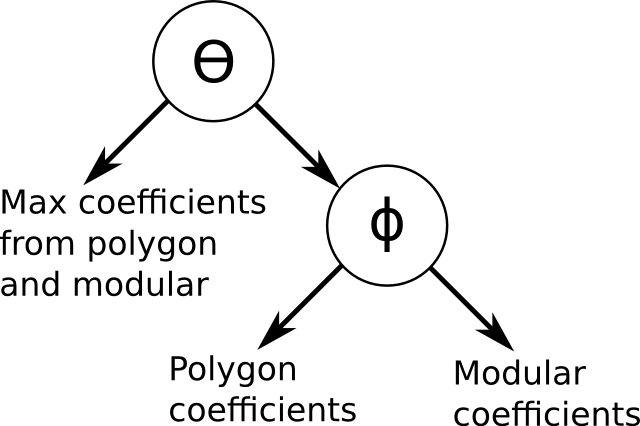
\includegraphics[width=0.5\textwidth]{figures/hierarchical_model_schematic.png}
\caption{Hierarchical model}
\label{hierarchicalmodel}

\end{figure}
Although we found the hybrid group did perform better than either the polygon or modular group individually, it did not seem to achieve truly best-of-both-worlds performance. One explanation for this might be that some subjects were just picking one representation and using it consistently, while others were really integrating both and performing optimally (at the maximal level of the two). We attempted to model this with a hierarchical model which assumed that the data were generated by the following process (depicted schematically in fig. \ref{hierarchicalmodel}): 
\begin{enumerate}
\item With probability $\theta$, the subject would integrate the material, and would perform optimally in the sense that their data would be best fit by assuming they picked the optimal representation on each question (or equivalently, that their regression coefficients were the element-wise maximum of the regression coefficients of the two other groups). 
\item If the subjects did not integrate (probability $1-\theta$), they would pick the polygon representation with probability $\phi$, and the modular representation with probability $1-\phi$, and their data would be best fit by the coefficients for the respective group.
\end{enumerate}
We fit this model to the experiment 2 data, and estimated that $\theta = 0.53, \phi = 0.38$ (log-likelihood $LL=-821.9$), so the data are best fit under this model by assuming that a little more than half the subjects are perfectly integrating, and those that aren't are choosing the modular representation over the polygon almost two-thirds of the time. We used the Aikake Information Criterion (AIC) to compare this model ($AIC = 1647.8$) to models where all subjects chose modular ($AIC=1829.6$), all chose polygon ($AIC = 1720.5$), where no subjects integrated i.e. a fixed $\theta = 0$ and fit $\phi = 0.65$ ($AIC = 1678.2$), and a model where all subjects integrated i.e. $\theta = 1.0$ ($AIC = 1689.9$). The full model is significantly better than any of these comparison models. However, there are many other possible ways people could use the two representations (such as picking arbitrarily on each question), so further investigation is needed.\par
Similarly, with the experiment 3 data we estimated that $\theta = 0.54, \phi = 0.61$ (log-likelihood $LL=-1782.3$), so the data are best fit under this model by assuming that a little more than half the subjects are perfectly integrating, and those that aren't are choosing the polyggon representation over the modular almost two-thirds of the time. We used the Aikake Information Criterion (AIC) to compare this model ($AIC = 3568.6$) to models where all subjects chose modular ($AIC=3826.5$), all chose polygon ($AIC = 3647.0$), where no subjects integrated, i.e. a fixed $\theta = 0$ and fit $\phi = 0.81$ ($AIC = 3612.8$), and a model where all subjects integrated, i.e. $\theta = 1.0$ ($AIC = 3613.8$). The full model is again significantly better than any of these comparison models. However, as above there are other possible ways that the subjects could use both representations, so there remain questions to be answered. Still, the consistent estimates of about 50\% integration suggest that they hybrid group is increasing the understanding of some subjects.\\
\subsubsection{Representation-Use Question Results}
For the experiment 3 representation-use questions, we performed logistic regressions predicting score on each representation-use question by the ratings ("Not at all" - "Very much", 5 point Likert scale) of representation used. We found that neither modular nor polygon rating was significantly predictive of success on the inverse of zero questions ($\beta_{mod} = -0.02$, $z = -0.15$, $p = 0.88$; $\beta_{poly} = 0.25$, $z = 1.37$, $p = 0.17$). We suspect this may have been due in part to the fact that this was the third presentation of an inverse of zero question, so subjects may have simply recalled the answer. Performance was very high in the hybrid group overall on this question, the majority of the subjects got the question right in the representation-use section, it had the only positive intercept of any of the representation-use regressions.\par 
Intriguingly, we found that both modular and polygon rating were significantly predictive of success on inverse of non-zero questions ($\beta_{mod} = 1.09$, $z = 2.95$, $p = 0.003$; $\beta_{poly} = 1.11$, $z = 2.94$, $p = 0.003$). This, together with the previous finding, seems suggestive of some integration occuring in the hybrid condition, such that the advantages of each representation are to some extent shared even when the other representation is used. 
\begin{figure*}
\centering
\begin{subfigure}[c]{0.45\textwidth}
\centering 
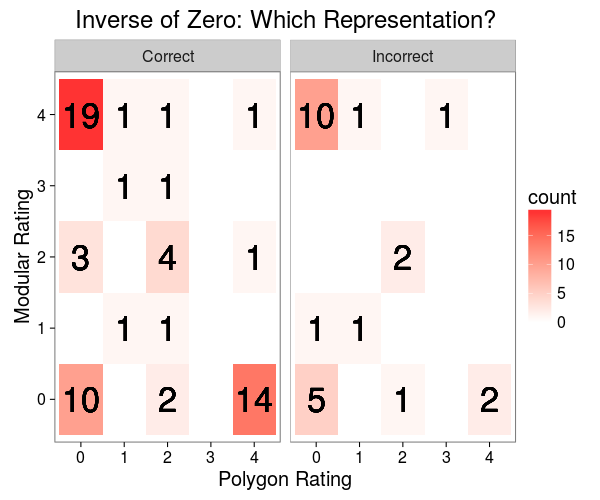
\includegraphics[width=\textwidth]{figures/3/wr_inZ.png}
\caption{Inverse of zero}
\end{subfigure}
~
\begin{subfigure}[c]{0.45\textwidth}
\centering 
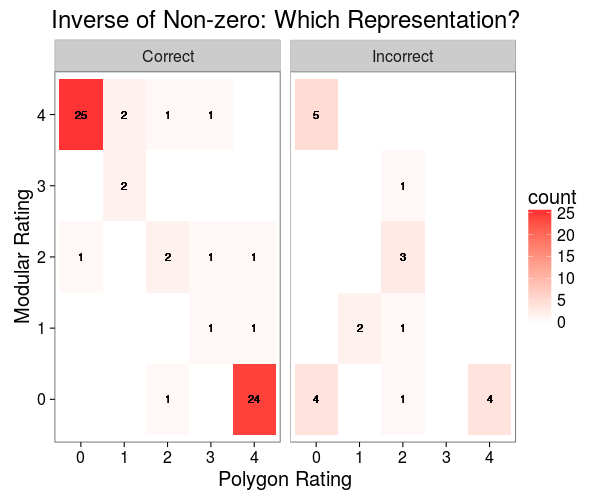
\includegraphics[width=\textwidth]{figures/3/wr_inNZ.png}
\caption{Inverse of non-zero}
\end{subfigure}
\caption{Experiment 3 -- representation-use responses on inverse questions (counts of subjects giving each rating, split by score)}
\label{ex3_wr_in}
\end{figure*}\noindent
We found that subjects polygon rating, but not modular, was significantly predictive of success on identifying generators ($\beta_{mod} = 0.19$, $z = 0.95$, $p = 0.34$; $\beta_{poly} = 0.75$, $z = 3.86$, $p < 0.001$). This corroborates our other data supporting the superiority of the polygon representation for these question, but suggests (as much of our earlier data did) that the integration in the hybrid condition is far from complete. We found that neither rating was significantly preditive of success on the generator True/False questions ($\beta_{mod} = 0.19$, $z = 1.28$, $p = 0.20$; $\beta_{poly} = 0.31$, $z = 1.38$, $p = 0.17$). This is perhaps unsurprising, since overall performance was low, and we observed inconsistent effects with these questions across our experiments.\\
\begin{figure*}
\centering
\begin{subfigure}[c]{0.45\textwidth}
\centering 
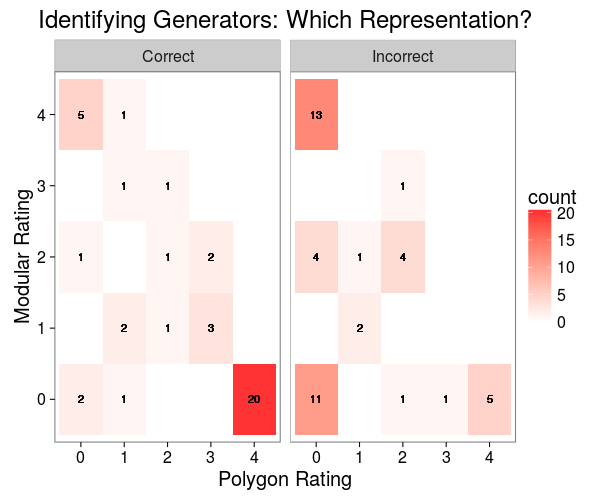
\includegraphics[width=\textwidth]{figures/3/wr_genT.png}
\caption{Identifying generators}
\end{subfigure}
~
\begin{subfigure}[c]{0.45\textwidth}
\centering 
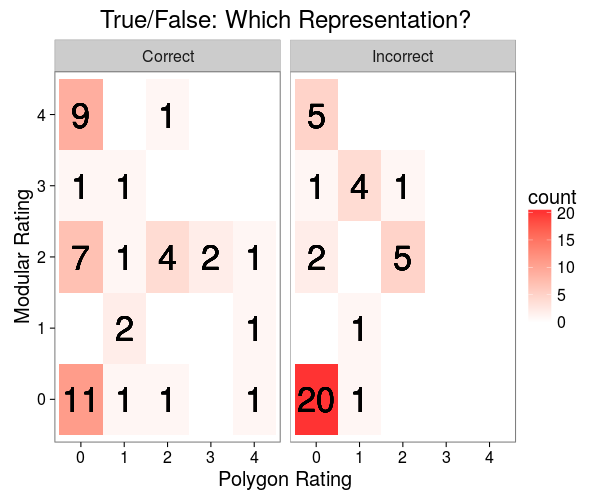
\includegraphics[width=\textwidth]{figures/3/wr_genTF.png}
\caption{Generator T/F}
\end{subfigure}
\caption{Experiment 3 -- representation-use responses on generator questions (counts of subjects giving each rating, split by score)}

\label{ex3_wr_gen}
\end{figure*}
\subsubsection{Analysis of hybrid subject word use}
We also attempted to investigate the hybrid subjects' use of different representations by the presence of words in their explanations that corresponded to one of the representations or another. First, we hand-crafted classifiers for the polygon and modular condition, respectively, based on the most common words that were specific to the condition (Polygon condition: move, spaces, clockwise, steps, arrow, hexagon, nonagon, ngon, spots, positions; Modular condition: add, subtract, plus, minus, +). We counted the occurrences of each of these words in each explanation, and then classified it as polygon if the polygon-word-count was higher, and as modular if the modular-word-count was higher. This produced highly specific, though not especially sensitive, classifiers for the conditions, see table \ref{wordusevaltable} for comparisons of classifier estimate of condition versus true condition across all questions with explanations in experiment 1. (Note that most of the failures here were cases where the subjects did not use words from either category.)
\begin{table} 
\centering
    \begin{subtable}[c]{0.5\textwidth}
	\centering
	\begin{tabular}{|r|c c|}
	    \hline   & not classified poly. & classified poly. \\ 
	    \hline actually mod. & 499 & 1 \\
	    actually poly. & 341 & 159 \\ \hline 
	\end{tabular}
	\caption{Polygon classifier}
    \end{subtable}
    \newline \vspace{1em}\newline 
    \begin{subtable}[c]{0.5\textwidth}
	\centering
	\begin{tabular}{|r|c c|}
	    \hline   & not classified mod. & classified mod. \\ 
	    \hline actually mod. & 380 & 120 \\
	    actually poly. & 496 & 4 \\ \hline 
	\end{tabular}
	\caption{Modular classifier}
    \end{subtable}
\caption{Validation of word-use classifiers}
\label{wordusevaltable}
\end{table} 
Using these classifiers on the hybrid data from experiment 2, we found that the hybrid subjects were classified as using more polygon words on 58 answers total across all questions for all subjects, and more modular words on 33 answers. We compared scores across classifier groups, and found some intriguing patterns, see table \ref{worduseresultstable}. On questions about the inverse of non-zero elements, hybrid subjects rated as using more polygon words appeared more accurate than those not using more polygon words, and those using more modular words appeared less accurate than those not using more modular words (table \ref{polyclassintable} \& \ref{modclassintable}). Similarly, on questions where they had to identify a generator, hybrid subjects rated as using more polygon words appeared more accurate than those not using more polygon words, and those using more modular words also appeared more accurate than those not using more modular words, but more subjects used polygon words than modular (table \ref{polyclassgentable} \& \ref{modclassgentable}). \par
\begin{table}
\centering
    \begin{subtable}[c]{0.5\textwidth}
	\centering
	\begin{tabular}{|r|c c|}
	    \hline   & score = 0 & score = 1 \\ 
	    \hline not classified polygon & 6 & 30 \\
	    classified polygon & 0 & 10 \\ \hline 
	\end{tabular}
	\caption{Inverse of non-zero questions: polygon classifier}
	\label{polyclassintable}
    \end{subtable}
    \newline \vspace{1em}\newline 
    \begin{subtable}[c]{0.5\textwidth}
	\centering
	\begin{tabular}{|r|c c|}
	    \hline   & score = 0 & score = 1 \\ 
	    \hline not classified modular & 4 & 37 \\
	    classified modular & 2 & 3 \\ \hline 
	\end{tabular}
	\caption{Inverse of non-zero questions: modular classifier}
	\label{modclassintable}
    \end{subtable}
    \newline \vspace{1em}\newline 
    \begin{subtable}[c]{0.5\textwidth}
	\centering
	\begin{tabular}{|r|c c|}
	    \hline   & score = 0 & score = 1 \\ 
	    \hline not classified polygon & 45 & 38 \\
	    classified polygon & 0 & 9 \\ \hline 
	\end{tabular}
	\caption{Generator questions: polygon classifier}
	\label{polyclassgentable}
    \end{subtable}
    \newline \vspace{1em}\newline 
    \begin{subtable}[c]{0.5\textwidth}
	\centering
	\begin{tabular}{|r|c c|}
	    \hline   & score = 0 & score = 1 \\ 
	    \hline not classified modular & 45 & 45 \\
	    classified modular & 0 & 2 \\ \hline 
	\end{tabular}
	\caption{Generator questions: modular classifier}
	\label{modclassgentable}
    \end{subtable}
\caption{Word-use classifier results}
\label{worduseresultstable}
\end{table} 
These results should not be read too strongly, because they are based on a few data points, because we did not ask for explanations on every question, and many subjects did not use specific words in their explanations. In part, this may be due to our design, by attempting to homogenize the language we used when presenting more advanced concepts to subjects, and remove references to the underlying operation, we implicitly encouraged subjects to give explanations that used representation-agnostic language (e.g. ``5 can make all the other elements'' instead of ``using 5 we can reach each other point on the nonagon''). We also tried using more general classifiers that were derived directly from the data, using the 20 or 40 most selective words and estimating the posterior probabilities from these, but while these classifiers were more sensitive, they were significantly less specific, so we think the interpretation of those results would be even more difficult. 
\section{Discussion}
\subsection{Polygon vs. Modular Representations}
Despite the fact that the polygon and modular groups did not significantly differ at learning the initial operation, they did differ in their ability to understand the subsequent concepts built upon it. Furthermore, one representation was not generally ``better'' than the other, they both had strengths and weaknesses (the polygon group performed better at identifying generators and finding the inverse of zero, the modular group performed better at finding the inverse of non-zero elements). Thus our initial hypothesis that there would be differences in performance between the groups was confirmed.\\ 
\subsubsection{Process Differences Underlying the Performance Differences}
Although we have not fully explored these factors, we do have some hypotheses for the pattern of results we observed, based on responses to problems where we asked the subjects to explain their answers as well as factors like explicit use of the diagram:\par 
\textit{Inverses:} It appears that the modular representation may have cued the subjects to recognize an algorithm for finding most of the inverses, namely that the inverse of $x$ can be found by subtracting $x$ from the group order. For example, under $+_6$, the inverse of $2$ is $4$, and $6-2 = 4$. This would not be as obvious for the polygon group, which mostly found inverses by counting, which is less reliable. However, the algorithm breaks down when $x = 0$, because the inverse of $0$ is $0$, not the group order. We suspect that subjects in the polygon group made more mistakes counting than the modular group on inverses of non-zero elements, but the modular group subjects were misled by this algorithm when computing the inverse of zero. \par
\textit{Generators:} There is a spatial structure to the generator questions in the polygon case which may assist in solving them, for example, when finding if $5$ is a generator on the nonagon, we get the sequence $5 \rightarrow 1 \rightarrow 4 \rightarrow 2 \rightarrow \cdots$. It might be more clear to someone seeing the polygon how precisely this sequence would fill in the gaps to generate all the numbers. This hypothesis is corroborated by our post-hoc analysis demonstrating that diagram use was predictive of success on these questions (more so than in the experiment overall). By contrast, for the formal questions in the order $n$ case, it is difficult or impossible to use these spatial intuitions, which would explain why the polygon group's advantage disappears.
\subsection{Hybrid Group}
The results from our meta-analysis suggest that by the time they reached the order 9 group, the hybrid group subjects were able to integrate their understanding to achieve approximately ``best of both worlds'' performance, in the sense that they outperformed the modular group where the polygon group was superior, and performed comparably to the modular group where it was superior. However, they did not appear to be achieving the full advantages of each group. Our hierarchical modeling results suggest that this imperfect performance may be explained by some individual variation, with some subjects integrating the representations better than others. \par 
In our analysis of the representation-use question responses, we also observed some heterogeneity in the overall integration. On some question types, such as finding the inverse of non-zero elements, it appears that the hybrid group has integrated sufficiently so that using either representation is equally beneficial. On others, such as identifying generators, one representation is still much more beneficial than the other for the hybrid group. This may reflect the underlying nature of the knowledge we think is being used for each of these scenarios. We hypothesized above that the modular formulation cues a process for finding the inverse of non-zero elements based on subtraction, which might be accessible using either representation. However, we posited that the advantages of polygon group on the identifying generator questions were based on a visuospatial reasoning process which could not as easily be transferred to the modular representation. \par 
It remains a question for future research how the strategy could be altered to encourage more uniform improvement across all question types and subjects. Nevertheless, these results at least begin to suggest that the use and integration of multiple representations may be beneficial to overall understanding. 
\subsection{Formalization}
None of the presentations seemed to encourage formalization particularly well, as evidenced by the low overall performance on the order $n$ group questions. (E.g., despite the fact that performance on the inverse questions was around 75\% on average, only about 25\% of the subjects were able to articulate the formula for computing an inverse in a generic cyclic group.) This may be because the length of the study was too short for the subjects process-level understanding to crystallize into a more formal understanding, or it may be representative of the more general separation between these aspects of understanding. Further research addressing these questions would be beneficial. 
\section{Conclusion}
We explored the way presentation of concepts in math instruction affects understanding of the concept being exemplified, and of more abstract concepts built upon it, using elementary group theory as our test domain. We found that even if two representations produce equal performance on a basic concept, they can produce differential understanding of the more abstract concepts related to it. Furthermore, it does not appear that there is always a clear advantage of one representation over another, instead a representation may be more useful for some concepts or some aspects of reasoning, and less useful for others. We think that these findings provide a contribution to the discussion of representation in math cognition, illustrating that representations have different advantages and disadvantages. This suggests that the pursuit of a single best type of representation may be futile. \par
Instead, we have identified an alternative strategy for improving performance: teaching multiple representations while encouraging subjects to integrate them. Preliminary data suggests that this may have positive effects even if the total instruction time is approximately the same. By the end of the experiment, subjects in our hybrid condition appeared to have integrated some of the material for a more holistic understanding, and to perform better overall than those instructed with one presentation alone. However, it remains to be seen whether they could truly achieve best-of-both-worlds performance over a longer time period, and whether this or another approach could encourage subjects to formalize their understanding. We think these questions provide an exciting new direction for research in both math cognition and math pedagogy.  
 
\bibliography{fyp_writeup_citations}

\bibliographystyle{apalike}

\setcounter{secnumdepth}{-1}
\clearpage
\section{Appendix A: A Brief, Selective Introduction to Group Theory}
Groups are mathematical structures that provide us with a nice way of doing something like arithmetic with things besides the ordinary numbers, like symmetries of an object or permutations, or with smaller sets of ordinary numbers (as in this paper). They have applications throughout mathematics, physics, chemistry, and computer science. Here I present the formal definition of a group with informal intuitions in italics. A \textbf{group} consists of a set $G$ (\emph{some objects}) and a binary operation $*: G\times G \rightarrow G$ (\emph{a way of combining two objects to get another object}) such that:  
\begin{itemize}
\item $G$ is \textbf{closed} under $*$, that is $a*b \in G$ for all $a,b \in G$. (\emph{Combining two of the objects you started with gives you another of the objects you started with.}) 
\item $*$ is \textbf{associative}, $a*(b*c) = (a*b)*c$ for all $a,b,c \in G$. (\emph{It doesn't matter how you parenthesize the operation, just like addition or multiplication.})
\item There is an \textbf{identity} element $e \in G$ such that $\forall x \in G, e*x = x*e = x$. (\emph{There's something that when you combine it with anything else has no effect, just like multiplying by one gives you the same number back.})
\item Each element $x \in G$ has an \textbf{inverse} element $x^{-1} \in G$ such that $x*x^{-1} = x^{-1}*x = e$. (\emph{There's something you can combine with each element to get back to the identity, just like $2 \times 0.5 = 1$.})
\end{itemize}
For example, if we take $G$ to be the numbers less than $4$, $G = \{0,1,2,3\}$, and define a new operation $*$ by $$a*b = \begin{cases} a+b & \text{if } a+b < 4 \\ a+b-4 & \text{if } a+b \geq 4 \end{cases}$$
$G$ and $*$ form a group, called the \textbf{cyclic group of order 4}. For example, in this group $1*1 = 2$, $2 * 3 = 5-4 = 1$ because $5 \geq 4$, $3*1 = 4-4 = 0$, etc. $0$ is the identity in this group, because $0*x = x*0 = x$ for any of $0,1,2,3$. Furthermore, the inverse of $1$ in the group is $3$, because $1*3 = 4-4 = 0$, the inverse of $2$ is $2$, and so on.\par
There is a great deal of structure to groups, far more than there is space to explain here. The only topic of interest for us beyond these simple properties will be the concept of \textbf{generators}. An element $x$ generates a group if every other element of the group can be written as $x*x*\cdots*x$ for some number of $x$s. For example, in our cyclic group of order 4, defined above, 1 is a generator of the group because $1 = 1, 2 = 1 * 1, 3 = 1 * 1 * 1, 0 = 1 * 1 * 1 * 1$. Similarly, 3 is a generator because $3 = 3, 2 = 3 * 3, 1 = 3 * 3 * 3, 0 = 3 * 3 * 3 * 3$. However, 2 is not a generator because $2 = 2, 0 = 2 * 2$, but there is no way to generate 1 or 3 using 2. This illustrates the only theorem we will give here: \par
\textbf{Cyclic Group Generators Theorem:} In a cyclic group of order $n$, written as the integers $0$ to $n-1$, $x < n$ generates the group if and only if $x$ and $n$ are relatively prime (i.e. have no common factors except 1). \par 
For more information on groups and group theory, see e.g. \cite{Lang2002}.
\onecolumn
\clearpage
\section{Appendix B: Full Result Plots}
\begin{figure}[H]
\centering
\begin{subfigure}[c]{0.3\textwidth}
\centering
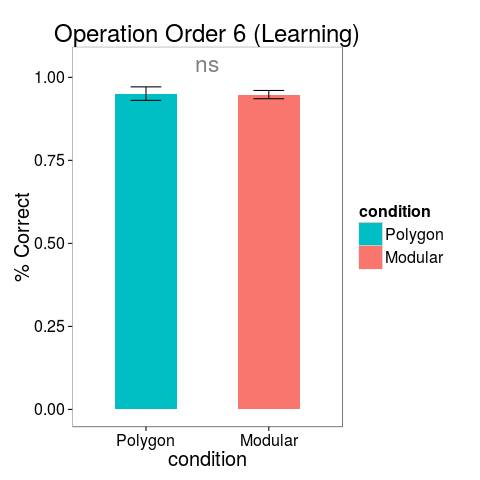
\includegraphics[width=\textwidth]{figures/1/op_6_r.png}
\end{subfigure}
~
\begin{subfigure}[c]{0.3\textwidth}
\centering
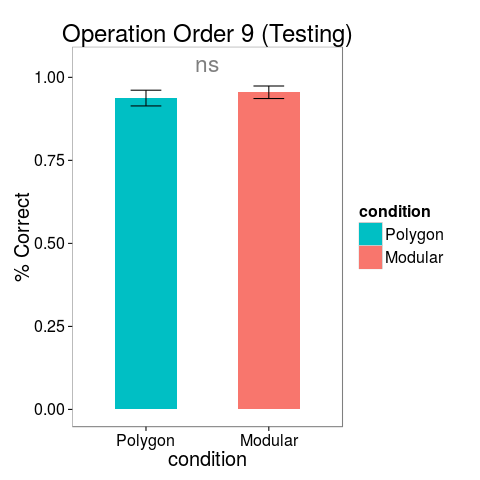
\includegraphics[width=\textwidth]{figures/1/op_9_r.png}
\end{subfigure}
\caption{Experiment 1 -- operation results}
\label{ex1_op}
\end{figure} 
\begin{figure}[H]
\centering
\begin{subfigure}[c]{0.3\textwidth}
\centering
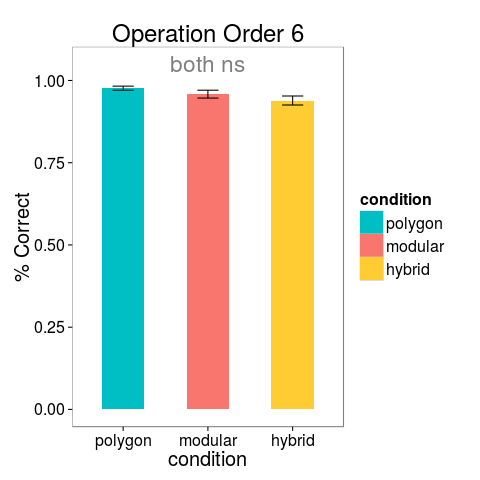
\includegraphics[width=\textwidth]{figures/2/op_6_r.png}
\end{subfigure}
~
\begin{subfigure}[c]{0.3\textwidth}
\centering
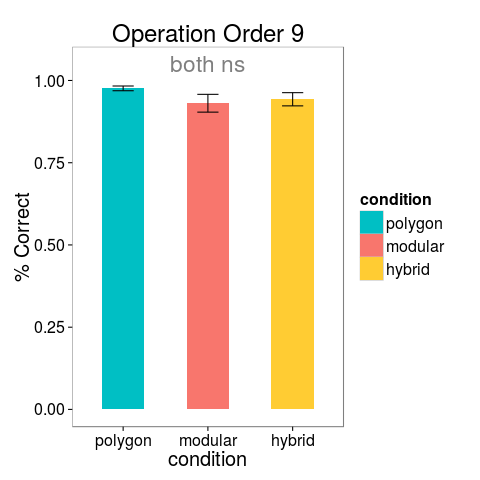
\includegraphics[width=\textwidth]{figures/2/op_9_r.png}
\end{subfigure}
\caption{Experiment 2 -- operation results}
\label{ex2_op}
\end{figure} 
\begin{figure}[H]
\centering
\begin{subfigure}[c]{0.3\textwidth}
\centering
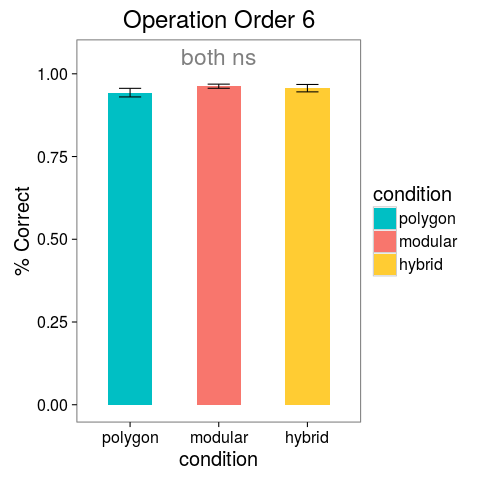
\includegraphics[width=\textwidth]{figures/3/op_6_r.png}
\end{subfigure}
~
\begin{subfigure}[c]{0.3\textwidth}
\centering
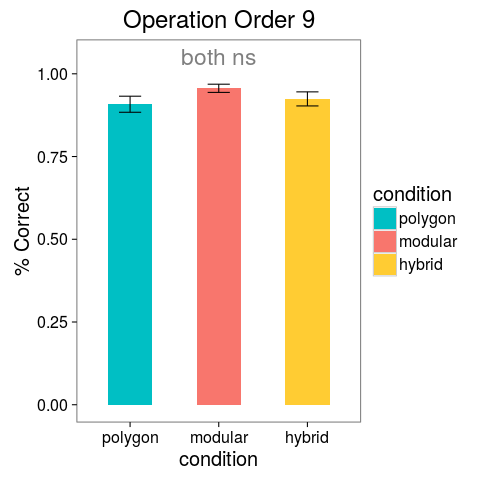
\includegraphics[width=\textwidth]{figures/3/op_9_r.png}
\end{subfigure}
\caption{Experiment 3 -- operation results}
\label{ex3_op}
\end{figure} 

\begin{figure}[H]
\centering
\begin{subfigure}[c]{0.3\textwidth}
\centering
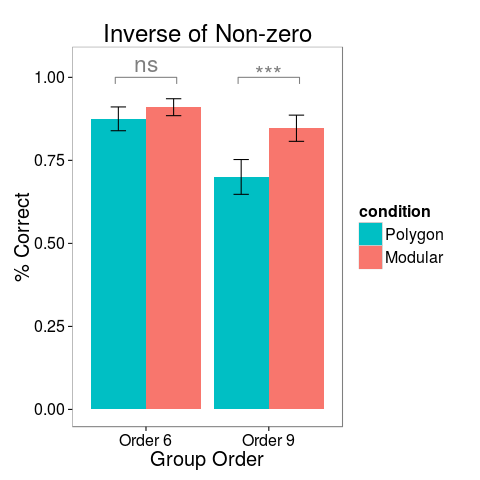
\includegraphics[width=\textwidth]{figures/1/in_NZ_r.png}
\end{subfigure}
~
\begin{subfigure}[c]{0.3\textwidth}
\centering
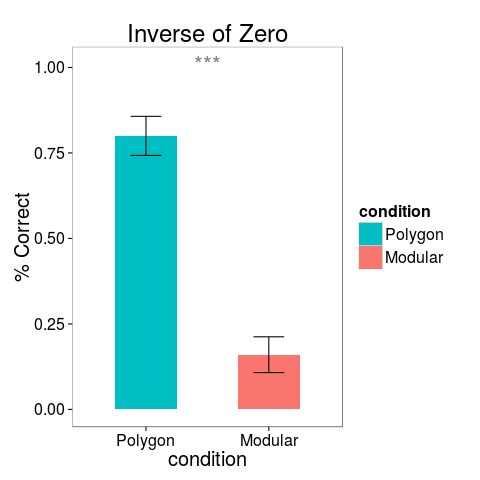
\includegraphics[width=\textwidth]{figures/1/in_Z_r.png}
\end{subfigure}
~
\begin{subfigure}[c]{0.3\textwidth}
\centering
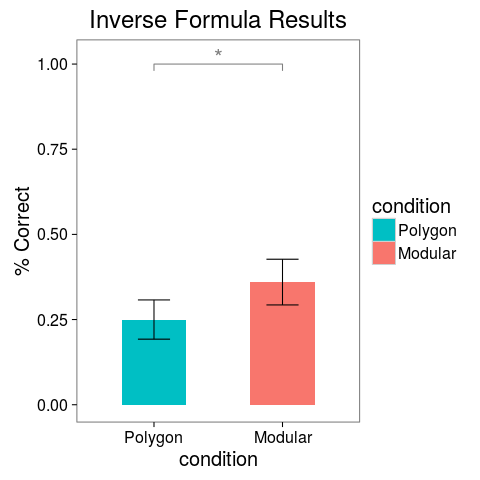
\includegraphics[width=\textwidth]{figures/1/in_f_r.png}
\end{subfigure}
\caption{Experiment 1 -- inverse results}
\label{ex1_in}
\end{figure}\noindent 
\begin{figure}[H]
\centering
\begin{subfigure}[c]{0.3\textwidth}
\centering
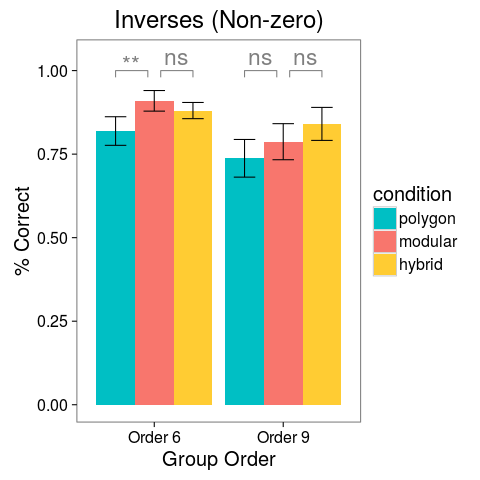
\includegraphics[width=\textwidth]{figures/2/in_NZ_r.png}
\end{subfigure}
~
\begin{subfigure}[c]{0.3\textwidth}
\centering
\includegraphics[width=\textwidth]{figures/2/in_Z_r.png}
\end{subfigure}
~
\begin{subfigure}[c]{0.3\textwidth}
\centering
\includegraphics[width=\textwidth]{figures/2/in_f_r.png}
\end{subfigure}
\caption{Experiment 2 -- inverse results}
\label{ex2_in}
\end{figure} 
\begin{figure}[H]
\centering
\begin{subfigure}[c]{0.3\textwidth}
\centering
\includegraphics[width=\textwidth]{figures/3/in_NZ_r.png}
\end{subfigure}
~
\begin{subfigure}[c]{0.3\textwidth}
\centering
\includegraphics[width=\textwidth]{figures/3/in_Z_r.png}
\end{subfigure}
~
\begin{subfigure}[c]{0.3\textwidth}
\centering
\includegraphics[width=\textwidth]{figures/3/in_f_r.png}
\end{subfigure}
\caption{Experiment 3 -- inverse results}
\label{ex3_in}
\end{figure} 

\begin{figure}[H]
\centering
\begin{subfigure}[c]{0.3\textwidth}
\centering
\includegraphics[width=\textwidth]{figures/1/gen_T_r.png}
\end{subfigure}
~
\begin{subfigure}[c]{0.3\textwidth}
\centering
\includegraphics[width=\textwidth]{figures/1/gen_F_r.png}
\end{subfigure}
\caption{Experiment 1 -- generator results}
\label{ex1_gen}
\end{figure}\noindent 
\begin{figure}[H]
\centering
\begin{subfigure}[c]{0.3\textwidth}
\centering
\includegraphics[width=\textwidth]{figures/1/gen_TF_r.png}
\end{subfigure}
~
\begin{subfigure}[c]{0.3\textwidth}
\centering
\includegraphics[width=\textwidth]{figures/1/gen_ASN_r.png}
\end{subfigure}
\caption{Experiment 1 -- generator T/F \& A/S/N results}
\label{ex1_TFASN}
\end{figure}\noindent 

\begin{figure}[H]
\centering
\begin{subfigure}[c]{0.3\textwidth}
\centering
\includegraphics[width=\textwidth]{figures/2/gen_T_r.png}
\end{subfigure}
~
\begin{subfigure}[c]{0.3\textwidth}
\centering
\includegraphics[width=\textwidth]{figures/2/gen_F_r.png}
\end{subfigure}
\caption{Experiment 2 -- generator results}
\label{ex2_gen}
\end{figure}\noindent 
\begin{figure}[H]
\centering
\begin{subfigure}[c]{0.3\textwidth}
\centering
\includegraphics[width=\textwidth]{figures/2/gen_TF_r.png}
\end{subfigure}
~
\begin{subfigure}[c]{0.3\textwidth}
\centering
\includegraphics[width=\textwidth]{figures/2/gen_ASN_r.png}
\end{subfigure}
\caption{Experiment 2 -- generator T/F \& A/S/N results}
\label{ex2_TFASN}
\end{figure}\noindent 

\begin{figure}[H]
\centering
\begin{subfigure}[c]{0.3\textwidth}
\centering
\includegraphics[width=\textwidth]{figures/3/gen_T_r.png}
\end{subfigure}
~
\begin{subfigure}[c]{0.3\textwidth}
\centering
\includegraphics[width=\textwidth]{figures/3/gen_F_r.png}
\end{subfigure}
\caption{Experiment 3 -- generator results}
\label{ex3_gen}
\end{figure}\noindent 
\begin{figure}[H]
\centering
\begin{subfigure}[c]{0.3\textwidth}
\centering
\includegraphics[width=\textwidth]{figures/3/gen_TF_r.png}
\end{subfigure}
~
\begin{subfigure}[c]{0.3\textwidth}
\centering
\includegraphics[width=\textwidth]{figures/3/gen_ASN_r.png}
\end{subfigure}
\caption{Experiment 3 -- generator T/F \& A/S/N results}
\label{ex3_TFASN}
\end{figure}\noindent 
\end{document} 
